\chapter{Linear Control Variates for Monte~Carlo \mbox{Estimation}}\label{ch:cvinsrns}
% \author{Michael Backenk\"ohler\inst{1}, Luca Bortolussi\inst{1,2}, Verena Wolf\inst{1}}
% \authorrunning{M.\ Backenk\"ohler et al.}
% \institute{\inst{1}Saarland University, Germany, \inst{2}University of Trieste, Italy}
% \maketitle
% \begin{abstract}
% Stochastic simulation is a widely used method for 
% estimating quantities in models of chemical 
% reaction networks where uncertainty plays a crucial role.
% However,  reducing  the statistical uncertainty of the corresponding  
% estimators requires the generation of a large number 
% of simulation runs, which is computationally expensive.
% To reduce the number of necessary runs, we propose a
% variance reduction technique based on control variates.
% We exploit  constraints on the statistical moments of the 
% stochastic process
% to reduce the estimators' variances.
% We develop an algorithm that selects appropriate control
% variates in an on-line fashion and demonstrate the efficiency of our approach  on several case studies.
% 
% \keywords{Chemical Reaction Network  \and Chemical Master Equation \and Stochastic Simulation Algorithm
% \and Moment Equations \and Control Variates \and Variance Reduction}
% \end{abstract}
% %
% %
%\section{Introduction}

Analysis approaches based on sampling, such as the \acf{SSA}~\parencite{gillespie1977exact}\turnto{sec:ssa}, can  be applied
independent of the size of the model's state-space. 
However, statistical approaches are costly since a large number
of simulation runs is necessary to reduce the statistical 
inaccuracy of estimators. This problem is particularly severe
if reactions occur on multiple time scales or if the event of interest is rare.
A particularly popular technique to speed up simulations is $\tau$-leaping which applies
multiple reactions in one step of the simulation.
However, such multi-step simulations rely on certain assumptions about
the number of reactions in a certain time interval. These assumptions
are typically only approximately fulfilled and therefore introduce  approximation
errors on top of the statistical uncertainty of the considered point estimators.

Moment-based techniques offer a fast approximation of the statistical moments of the model. 
The exact moment dynamics can be expressed as an infinite-dimensional system of \acp{ODE}, which cannot be directly  integrated for a transient analysis.
Hence, ad-hoc approximations need to be introduced, expressing higher order moments as functions of lower-order ones \parencite{ale2013general,engblom2006computing}.
However, moment-based approaches rely on assumptions about the dynamics that are
often not even approximately fulfilled and may lead to high approximation errors. 
Recently, equations expressing the moment dynamics have also been used as constraints for parameter
estimation \parencite{backenkohler2018moment} and for computing moment bounds using semi-definite programming \parencite{dowdy2018dynamic,ghusinga2017exact}.

In this work, we propose a combination of such moment constraints with the \ac{SSA} approach.
Specifically, we   interpret these constraints as random variables 
that are correlated with the estimators of interest usually given as functions of chemical population variables.
These constraints can be used  as  (linear) \acfp{CV} in order to improve the final estimate and reduce its variance \parencite{lavenberg1982statistical,szechtman2003control}.
The method is easy on an intuitive level: If a control variate
is positively correlated with the function to be estimated then 
we can use the estimate of the variate to
adjust the target estimate.
%more details

The incorporation of control variates into the \ac{SSA}
introduces   additional simulation costs for the calculation of the constraint values.
These values are integrals over time, which we accumulate  based on the
piece-wise constant trajectories.
This introduces a trade-off between the variance reduction that is achieved
by using control variates versus the increased simulation cost.
This trade-off is expressed as the product of the variance reduction ratio
and the cost increase ratio.

For a good trade-off, it is crucial to find an appropriate set of control variates.
Here we propose a class of constraints which is parameterized by a moment vector
and a weighting parameter, resulting in infinitely many choices.
We present an algorithm that samples from the set of all constraints and
proceeds to remove constraints that are either only weakly correlated with the
target function or are redundant in combination with other constraints.

In a case study, we explore different variants of this algorithm
both in terms of generating the initial constraint set and of
removing  weak or redundant constraints.
We find that the algorithm's efficiency is superior to a standard estimation procedure
using stochastic simulation alone
in almost all cases.

Although in this work we focus on  estimating first order moments at
fixed time points, the proposed approach can in principle deal with any property that can
be expressed in terms of expected values such as probabilities
of complex path properties.
Another advantage of our technique is that an increased efficiency is achieved without the price of an additional approximation error as it is the case for methods based on moment approximations or multi-step simulations.

\section{Related Work}\label{sec:cv:related}
\paragraph{State-space Truncations}
If the state-space is finite and small enough one can deal with the underlying Markov
chain directly.
But there are also  cases where the transient distribution has an infinitely large support
and one can still deal with explicit state probabilities.
To this end, one can fix a finite state-space, that should contain most of the
probability~\parencite{munsky2006finite}. Refinements of the method work
dynamically and adjust the state-space according to the transient
distributions~\parencite{andreychenko2011parameter,henzinger2009sliding,mateescu2010fast}.

\paragraph{Moment Approximations}
On the other end of the spectrum there are mean-field approximations, 
which model the mean densities faithfully in the system size limit~\parencite{bortolussi2013continuous}.
In between there are techniques such as moment closure \parencite{singh2006lognormal}, that
not only consider the mean, but also the variance and other higher order moments.
These methods depend on ad-hoc approximations of higher order moments to
close the \ac{ODE} system given by the moment equations.
Yet another class of methods approximate molecular counts continuously and approximate the dynamics in such a continuous space, e.g. the system size expansion~\parencite{van1992stochastic} and the
chemical Langevin equation~\parencite{gillespie2000chemical}.

While the moment closure method uses ad-hoc approximations for high order moments to
facilitate numerical integration, they can be avoided in some contexts.
For the equilibrium distribution, for example, the time-derivative of all moments is equal to zero.
This directly yields constraints that have been used for parameter estimation at
steady-state~\parencite{backenkohler2018moment}
and bounding moments of the equilibrium distribution using semi-definite
programming~\parencite{ghusinga2017estimating,ghusinga2017exact,kuntz2017rigorous}.
The latter technique of bounding moments has been successfully adapted in the 
context of transient analysis~\parencite{dowdy2018dynamic,sakurai2017convex,sakurai2019bounding}.
We adapt the constraints proposed in these works to improve statistical estimations via stochastic
simulation (cf.\ \autoref{sec:cv:moments}).


\paragraph{Monte Carlo Simulation}
While the above techniques give a deterministic output, stochastic simulation generates
single executions of the stochastic process~\parencite{gillespie1977exact}.
This necessitates accumulating large numbers of simulation runs to estimate
quantities.
This adds a significant computational burden. Consequently, considerable effort
has been directed at lowering this cost.
A prominent technique is $\tau$-leaping~\parencite{gillespie2001approximate},
which in one step performs multiple instead of only a single reaction.
Another approach is to find approximations that are specific to the problem at hand,
such as approximations based on time-scale separations~\parencite{cao2005slow,bortolussi2015efficient}.

Recently, multilevel Monte Carlo methods have been applied in to time-inhomogenous
\ac{MPM}~\parencite{anderson2018low}. In this techniques estimates are combined
using estimates of different approximation levels.

% \parencite{goodman2009coupling}

The most prominent application of a variance reduction technique in the context
of stochastic reaction networks is importance sampling~\parencite{kuwahara2008efficient}.
This technique relies on an alteration of the process and then weighting samples
using the likelihood-ratio between the original and the altered process.
% \vw{This sentence stands here a bit lonely. Maybe shortly explain importance sampling? Also: there are papers about importance splitting (does this count as variance reduction technique? I would guess so.)}
% 

% \vw{Warum sagst Du hier nicht kurz etwas über numerische Lösungen der CME und die Schwierigkeiten? Eigentlich wäre numerische Lösung vorzuziehen wenn sie nicht so schwierig wäre}




\section{Moment Constraints}\label{sec:cv:moments}
The time-evolution of $\E{f(X_t)}$ for some function $f$ is given by \eqref{eq:mom_ode}\turnto{eq:mom_ode}.
The integration of \eqref{eq:mom_ode} with such functions $f$ is well-known in the context of
moment approximations of \ac{MPM}.
For most models the arising \ac{ODE} system is infinitely large, because the time-derivative of
low order moments usually depends on the values of higher order moments.
To close this system, \emph{moment closures}, i.e.\ ad-hoc approximations of higher order moments
are applied \parencite{schnoerr2015}.
The main drawback of this kind of analysis is that it is not known whether the chosen closure gives
an accurate approximation for the case at hand.
Here, such approximations are not necessary, since we will apply the moment dynamics in the context
of stochastic sampling instead of trying to integrate \eqref{eq:mom_ode}.

Apart from integration strategies,
setting \eqref{eq:mom_ode} to zero has been used as a constraint for parameter estimation at steady-state
\parencite{backenkohler2018moment} and bounding moments at steady-state~\parencite{dowdy2018bounds,ghusinga2017exact,kuntz2017rigorous}.
The extension of the latter has recently lead to the adaption of these constraints
to a transient setting~\parencite{dowdy2018dynamic,sakurai2019bounding}.
These two transient constraint variants are analogously derived by multiplying \eqref{eq:mom_ode}
by a time-dependent, differentiable weighting function $w(t)$ and integrating:

As in the previous chapter,\turnto{eq:exp_constraint} multiplication with $w(t)$ and integration on $[t_0, T]$ yields~\parencite{dowdy2018dynamic,sakurai2019bounding}
\begin{multline}\label{eq:poly_con}
        w(T)\E{f(X_{T})}
        - w(t_0)\E{f(X_{t_0})}
	- \int_{t_0}^{T}\frac{dw(t)}{dt}\E{f(X_t)}\,dt\\
        =\sum_{j=1}^{n_R}\int_{t_0}^{T}w(t)
        \E{\left(f{(X_t + v_j)} - f(X_t)\right)\alpha_j(X_t)}\,dt
\end{multline}
While many choices of $f$ are possible, for this work we will restrict ourselves to
monomial functions $f(x)=x^m$, $m\in\mathbb{N}^{n_S}$
% \vw{ich dachte, m soll ein Vektor sein}
i.e.\ the \emph{non-central} or \emph{raw moments} of the process.
In the context of computing moment bounds via semi-definite programming
the polynomial $w(t)=t^s$~\parencite{sakurai2019bounding} and the exponential $w(t)=e^{\lambda(T - t)}$~\parencite{dowdy2018dynamic}
have been proposed.
While both choices proved to be effective in different case studies, relying solely on the latter choice,
i.e.\ \[
	w(t)=e^{\lambda(T - t)} \] was sufficient.
\marginpar{In \autoref{ch:MFPT} we chose the monomial, such that \eqref{eq:poly_con} would admit the interpretation of temporal moments. Here the exponential is a good choice, because it can model both increasing and decreasing weighting.}

% Let $$
% % \hat m^{(s)}_f = \int_{t_0}^{T}t^s\E{f(X_t)}\,dt
% % \quad\text{and}\quad
%  {m}^{(\lambda)}_f = \int_{t_0}^{T}e^{\lambda(T - t)}\E{f(X_t)}\,dt\,.
% $$
% We can interpret the constraint value as a random variable $Z$.
% Assuming $f$ and the rate functions are polynomials in $x$ we obtain\vw{der Schritt geht fuer mich zu schnell. Wie genau ist Z definiert?}
% \begin{equation}\label{eq:simpl_pol}
%     \E{Z_p} =\,
%          T^s\E{f(X(T))}
%         - t_0^s\E{f(X(t_0))}
%         - s\hat m^{(s-1)}_f
%         + \sum_{k}c_k\hat{m}^{(s)}_{f_k}
% \end{equation}
% and
% \begin{equation}\label{eq:simpl_exp}
%     \E{Z} =\,
%          \E{f(X(T))}
%         - e^{\lambda T}\E{f(X(t_0))}
%         % + \lambda m^{(\lambda)}_f
%         + \sum_{k}c_k{m}^{(\lambda)}_{f_k}\,,
% \end{equation}
By expanding the rate functions and $f$ in \eqref{eq:poly_con} and substituting the
exponential weight function we can re-write \eqref{eq:poly_con} as
\begin{multline}\label{eq:simpl_exp}
        0 =\,
         \E{f(X_{T})}
        - e^{\lambda T}\E{f(X_{t_0})}\\
        + \sum_{k}c_k\int_{t_0}^{T}e^{\lambda(T-t)}\E{X_t^{m_k}}\,dt
\end{multline}
with coefficients $c_k$ and vectors $m_k$ defined accordingly.
Assuming the moments remain finite on $[0,T]$, we can define the random variable
\begin{equation}\label{eq:z}
        Z =\,
         f(X_{T})
        - e^{\lambda T}f(X_{t_0})
        + \sum_{k}c_k\int_{t_0}^{T}e^{\lambda(T-t)}X_t^{m_k}\,dt
\end{equation}
with $\E{Z}=0$.
% Clearly, for $\rho=0$ and $z=0$ \eqref{eq:simpl_pol} and \eqref{eq:simpl_exp}
% are equivalent.
\begin{example}
For \autoref{model:bd} the moment equation for $f(x)=x$ becomes
% \vw{sollte -delta Ex sein}
	\[
		\frac{d}{dt}\E{X_t}=\gamma - \delta\E{X_t}\,.
	\]
The corresponding constraint \eqref{eq:simpl_exp} with $\lambda=0$ gives
	\[
		0=\E{X_T} - \E{X_0} - \gamma T + \delta \int_0^{T} \E{X_t}\,dt\,.
	\]
In this instance the constraint  leads to an explicit function of
the moment over time. If  $X_0=0$ w.p.\ $1$, then \eqref{eq:simpl_exp} becomes
\begin{equation}\label{eq:bd_constraint}
\E{X_T} = \frac{\gamma}{\delta} \left(1 - e^{-\delta T}\right)
\end{equation}
when choosing $\lambda=-\delta$.
% When we use this constraint as a control variate
% for the estimation of the mean at some time point, it has a correlation of $\pm1$.
% Therefore the variance is reduced to zero. This illustrates the benefit of choosing 
% control variates, that are highly correlated with the random variable of interest.
\end{example}


In general, a realization of $Z$ depends on the whole trajectory $\tau=x_0t_1 x_1 t_2 \dots\allowbreak t_n x_n$ over $[t_0,T]$.
Thus, for the integral terms
in \eqref{eq:z} we have to compute sums
\begin{equation}\label{eq:dis_int}
    % \frac{1}{k+1}\sum_{i=1}^n\left(t_{i+1}^{k+1} - t_i^{k+1}\right)s_i^m
    % \quad\text{and}\quad
    \frac{1}{\lambda}\sum_{i=1}^n\left(e^{\lambda(T - t_{i+1})}
    - e^{\lambda(T-t_i)}\right)x_i^{m_k}
\end{equation}
over a given trajectory.
This accumulation is best done during the simulation to avoid storing the whole trajectory.
Still, the cost of a simulation run increases.
For the method to be efficient, the variance reduction (\autoref{sec:cv:var_red}) needs
to overcompensate for this increased cost of a simulation run.
\begin{algorithm}
    \SetKwInOut{Input}{input}
    \SetKwInOut{Output}{output}
    \Input{$\pi_0, T, P, n$}
    \Output{trajectory $\tau$}
    initialize accumulator map $A$ for $P$\;
    \For{$i=1,\dots, n$}{
        $\tau \leftarrow$ empty list, $s\leftarrow$ sample from $\pi_0$, $t\leftarrow 0$\;
        \While{$t<T$}{
        $\tau\leftarrow \text{append}(\tau, (s, t))$\;
            $k\leftarrow$ sample reaction $i$ with probability $\propto\alpha_i(s)$\;
            $\delta\sim \text{Exp}\left(\sum_i \alpha_i(s)\right)$\;
            \For{$(m,\lambda)\in \mathit{keys}(A)$}{
                $A[(m,\lambda)]\leftarrow A[(m,\lambda)] $\\ \hspace*{6em}$+\frac{1}{\lambda}\left(e^{ \lambda(t + \delta)} - e^{ \lambda t }\right)x^m$\;
            }
            $s\leftarrow s + v_k$\;
            $t \leftarrow t + \delta$\;
        }
        update means $\hat{V}$, $\hat{Z}$ and covariances $\hat\Sigma$ using $A$\;
        \For{$(m,\lambda)\in \mathit{keys}(A)$}{$A[(m,\lambda)] \leftarrow 0$}
    }
    \textbf{return} $(\hat{\Sigma},\hat{V}, \hat{Z})$\;
    \caption{\label{alg:ssa_lcv}$\text{SSA}_{\text{CV}}$: \ac{SSA} with accumulator updates}
\end{algorithm}

\section{Control Variates}\label{sec:cv:var_red}
Now, we are interested in the estimation of some quantity $\E{V}$
by stochastic simulation.
Let $V_1,\dots,V_n$ be independent samples of $V$.
Then the sample mean 
\[
	\hat{V}_n =\frac{1}{n}\sum_{i=1}^n V_k
\]
is an estimate of $\E{V}$.  By the central limit theorem
\[
\sqrt{n}\hat{V}_n\xrightarrow{d}N(\E{V},\sigma_V^2)\,.
\]
Now suppose, we know of a random variable $Z$ with $0=\E{Z}$.
The variable $Z$ is called a \emph{\acf{CV}}.
If a \acl{CV} $Z$ is correlated with $V$, we can
use it to
reduce the variance of $\hat{V}_n$~\parencite{glasserman2005large,nelson1990control,szechtman2003control,wilson1984variance}.
For example, consider we are running a set of simulations and consider a single
constraint.
If the estimated value of this constraint is larger than zero and we estimate a positive correlation
between the constraint $Z$ and $V$, we would, intuitively, like to {decrease} our
estimate $\hat{V}_n$ accordingly.
This results in an estimation of the mean of the random variable
\[
	Y_{\beta}= V-\beta Z
\]
instead of $V$.
The variance%\vw{wo kommt das alpha her?Sollte beta sein}
\[
	\sigma_{Y_{\beta}}^2 = \sigma_V^2-2\beta \Cov{V}{Z} + \beta^2\sigma_Z^2\,.
\]
The optimal choice $\beta$ can be computed by  considering the minimum of $\sigma_{Y_\beta}^2$. Then
\[
	\beta^{*}={\Cov{V}{Z}}/{\sigma_Z^2}\,.
\]
Therefore 
\[
	\sigma_{Y_{\beta^{*}}}=\sigma_Z^2(1 - \rho_{VZ}^2)\,,
\]
where $\rho_{VZ}$ is the correlation of $Z$ and $V$.

If multiple control variates are available, we can proceed in a similar fashion.
Now, let ${Z}$ denote a vector of $d$ control variates and let
\[
\Sigma=
\begin{bmatrix}
\Sigma_{ Z} & \Sigma_{V Z}\\
\Sigma_{ Z V} & \sigma_V^2
\end{bmatrix}
\]
be the covariance matrix of $({Z},V)$.
As above, we estimate the mean of
\[
    {Y}_{\beta}=V -{\beta}^{\T}{Z}\,.
    \]
The ideal choice of $\beta$ is the result of an ordinary least squares regression between $V$
and $Z_i$, $i=1,\dots,n$.
Specifically,
\[
	\beta^{*}={\Sigma_{ Z}}^{-1}{\Sigma}_{ Z V}\,.
\]
Then, asymptotically
the variance of the estimator
\begin{equation}
\hat{Y}_{{\beta^*}}=\hat{V}-{\beta^*}^{\top}\hat{ Z}
\end{equation}
is~\parencite{szechtman2003control},
\begin{equation}\label{eq:lcv_asym}
    {\sigma_{\hat Y_{\beta^*}}^2} = (1 - R_{ Z V}^2){\sigma_{\hat V}^2}\,,
\end{equation}
where
\begin{equation*}
    R_{ Z V}^2=\Sigma_{ Z V}\Sigma_{ Z}^{-1}\Sigma_{ Z V} / \sigma_V^2\,.
\end{equation*}
In practice, however, $\beta^*$ is unknown and needs to be replaced by
an estimate $\hat{\beta}$.
Then the estimator
\begin{equation}
\hat{Y}_{\hat{\beta}}=\hat{V}-\hat{\beta}^{\top}\hat{ Z}\,.
\end{equation}
This leads to an increase in the estimator's variance.
Under the assumption of $Z$ and $V$ having a multivariate normal
distribution~\parencite{cheng1978analysis,lavenberg1982statistical}, the variance of the estimator is
\begin{equation}\label{eq:lcv_norm_varred}
    {\sigma_{\hat{Y}_{\hat{\beta}}}^2} = \frac{n - 2}{n - 2 - d}(1 - R_{ ZV}^2){\sigma_{\hat V}^2}\,.
\end{equation}

Clearly, a control  variate is ``good'' if it is highly correlated with $V$.
The constraint in \eqref{eq:bd_constraint} is an example of the extreme case.
When we use this constraint as a control variate
for the estimation of the mean at some time point $t$, it has a correlation of $\pm1$
since it describes the mean at that time precisely.
Therefore the variance is reduced to zero.
We thus aim to pick control  variates that are highly correlated with $V$.

\begin{example} Consider, for example, the above case of the birth-death process.
If we choose \eqref{eq:bd_constraint} as a constraint, it would always yield
the exact difference of the exact mean to the sample mean and therefore have a 
	perfect correlation. Clearly, $\hat\beta$ reduces to \num{1} and $\hat Y_1 = \E{X_t}$.
\end{example}

\section{Moment-Based Variance Reduction}\label{sec:cv:algo}
We propose an adaptive estimation algorithm (\autoref{alg:ssa:lcv}) that starts out with
an initial set of control variates
and periodically removes potentially inefficient variates.
The ``accumulator set'' $A$ represents the time-integral terms \eqref{eq:dis_int}.
The size of $A$ has the most significant impact on the overall speed of the algorithm
since it represents the only factor incurring a direct cost increase in the \ac{SSA} itself (\autoref{line:run_ssa}).

The algorithm consists of a main loop which performs $n$ simulation runs (\autoref{line:main_loop}).
Between each run the mean and covariance estimates of $[Z,\;  V]$ are updated (\autoref{line:updates}).
Every $d<n$ iterations, the control variates are checked for  \emph{efficiency}
and \emph{redundancy} (lines \ref{line:cond_ck_begin}--\ref{line:cond_ck_end}).
\begin{figure}[htb]
	\centering
	\subfloat[$\E{X^A_2}$ in \autoref{model:dim}]
	{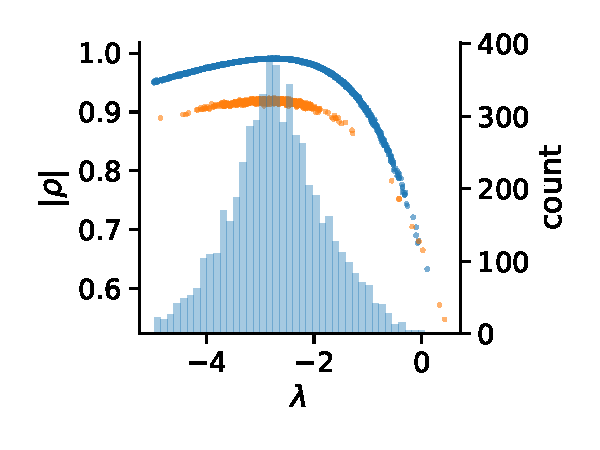
\includegraphics[scale=0.55]{gfx/cs_bdim.pdf}}
	\subfloat[$\E{X^X_{50}}$ in \autoref{model:dm}]
	{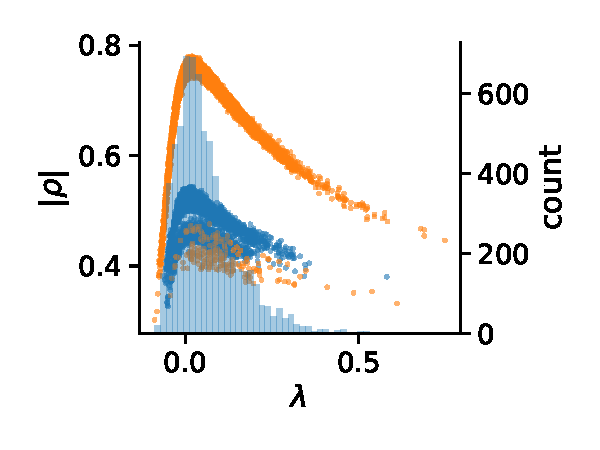
\includegraphics[scale=0.55]{gfx/cs_pm.pdf}}
	\caption[\ac{CV} correlation charactersitics]{The absolute correlation of different constraints {to $V$}
    arising from different choices of $\lambda$. The blue dots represent constraints
    based on first order moments, while the orange refers to control  variates derived from second
	order moments. In both cases $\num{10000}$ samples were used with
	\num{30} initial samples for $\lambda$ from $N(0,1)$ and $k_{\min}=2$. A quadratic decision bound was used for
    the redundancy removal. Furthermore, a histogram of control  variates selected by \autoref{alg:ssa:lcv}
    is given.
    In (a) $\E{X^A_2}$ in the dimerization model was estimated.
    In (b) $\E{X^X_{50}}$ in the distributive modification model was estimated.
    }
    \label{fig:bdim}
\end{figure}

Checking both conditions is based on the correlation $\rho_{ij}$ between the $i$-th and $j$-th control variate
and the correlation $\rho_{iv}$ of a control variate $i$ to $V$.
These are elements of the correlation matrix
\[
C=
\begin{bmatrix}
1 & \dots & \rho_{1k} & \rho_{1v} \\
\vdots & \ddots & \vdots & \vdots \\
\rho_{k1} & \dots & 1 & \rho_{kv} \\
\rho_{v1} & \dots & \rho_{vk} & 1
\end{bmatrix}\,.
\]
The first condition is a simple lower threshold $\rho_{\min}$ for a correlation $\rho_{iv}$.
This condition aims to remove those variates  from the control  variate set that are only weakly correlated to $V$ (\autoref{line:weak_covs}).
The rationale is that, if variate $i$ has a low correlation with the variable of interest $V$,
its computation may not be worth the costs.
Here, we propose to set $\rho_{\min}$ heuristically as
\[
	\rho_{\min} = \min\left(0.1, \frac{\max_{i}\rho_{iv}}{k_{\min}}\right)\,,
\]
where $k_{\min}>1$ is an algorithm parameter.

The second condition aims to remove redundant conditions.
This is not only beneficial for the efficiency of the estimator, but also 
necessary for the matrix inversion \eqref{eq:lcv_asym}
because perfectly and highly correlated constraints will make
the covariance matrix estimate $\hat{\Sigma}_Z$ (quasi-) singular.
For all considered criteria we iterate over all tuples $(i,j)\in \{1,\dots,k\}^2$, $i\neq j$,
removing the weaker of the two, i.e.\ $\argmin_{k\in\{i,j\}}\rho_{kv}$,
if the two control  variates are considered redundant (\autoref{line:redundant_covs}).

There are many ways to define such a redundancy criterion.
Here, we focus on criteria that are defined in terms of the
average correlation \[ \bar\rho_{ij}=(\rho_{iv} + \rho_{jv})/2\,.\]
For two variates $i$ and $j$ we then check if their mutual correlation
$\rho_{ij}$ exceeds a some function $\phi$ of ${\bar{\rho}}_{ij}$,
i.e.\ we check the inequality
\[
	\phi(\bar\rho_{ij}) \leq \rho_{ij}\,.
\]
If this inequality holds, constraint $\argmin_{k\in\{i,j\}}\rho_{kv}$ is removed.
Naturally, there are many possible choices for the above decision boundary $\phi$ (cf.\ \autoref{fig:decision}).


The simplest choice is to ignore $\bar\rho_{ij}$ and just fix a constant close to $1$ as a threshold,
e.g.\ \[ \phi_c(\bar\rho_{ij})=0.99\,.\] While this often leads to the strongest variance reduction
and avoids numerical issues in the control variate computation, it turns out
that the computational overhead is not as well-com\-pen\-sa\-ted as by other choices of $\phi$ (see \autoref{sec:cv:study}).

Another option is to fix a simple linear function, i.e.\ \[ \phi_{\ell}(\bar\rho_{ij})=\bar\rho_{ij}\,.\]
For this choice the intuition is, that one of two constraints is removed if their mutual
correlation exceeds their average correlation with $V$.


Here, we also assess two quadratic choices for $\phi$. The first choice of
\[
	\phi_{q}(\bar\rho)=1 - (1-\bar\rho)^2
\]
is more tolerant than the linear function and more strict than a threshold function, except for
highly correlated control  variates.
Another variant of $\phi$ is given by including the lower bound $\rho_{\min}$ and scaling
the quadratic function accordingly:
\[ \phi_{\mathit{sq}}(\bar\rho)=1-((1-\bar\rho)/(1-\rho_{\min}))^2\,.\]
The different choices of $\phi$ considered here are plotted in \autoref{fig:decision}.
\begin{algorithm}[ht]
\SetKwInOut{Input}{input}
\SetKwInOut{Output}{output}
\Input{$n, d, n_{\max}, n_{\lambda}, k_{\min}$}
\Output{an estimate using linear control variates}
  $L\leftarrow\{\lambda_i\sim \pi_\lambda \mid 1\leq i< n_{\lambda} \} \cup \{ 0 \}$\label{line:lambda_sample}\;
  $P \leftarrow \{ ({m}, \lambda) | 1\leq\lvert {m} \rvert \leq n_{\max}, \lambda\in L\}$\label{line:init_covs}\;
  \For{$i=1,\dots,\lfloor n/d \rfloor$\label{line:main_loop}}{
      $(\hat{\Sigma}_i, \hat{V}_i, \hat{Z}_i) \leftarrow \text{SSA}_{\text{CV}}(\pi_0,T,P,d)$\label{line:run_ssa}\;
     update $\hat\Sigma$, $\hat{V}$, and $\hat{Z}$\label{line:updates}\;
  		$\rho_{\min}\leftarrow \min\left(0.1,{\max_i \rho_{iv}}/{k_{\min}}\right)$\label{line:cond_ck_begin}\;
  		$P\leftarrow P\setminus\{({m}_k, \lambda_k)\mid \rho_{kv} < \rho_{\min}\}$\label{line:weak_covs}\;
  		$P\leftarrow P\setminus\{({m}_k, \lambda_k)\mid \exists i,j.i\neq j,
  		\phi(\bar\rho_{ij}) < \rho_{ij},$ \label{line:redundant_covs}\\
		\hspace{10em}$k=\argmin_{k\in\{i,j\}}\rho_{kv}\}$\label{line:cond_ck_end}\;
  	}
% % \State $\hat{\beta}\leftarrow\hat\Sigma_{{Z}}^{-1}\hat\Sigma_{{Z}V}$
\Return $\hat{V} - {(\hat{\Sigma}_{{Z}}^{-1}\hat\Sigma_{{Z}V})}^{\top}\hat{{Z}}$\label{line:compute_lcv}\;
    \caption{\label{alg:ssa:lcv}Estimate the mean of species $i$ at time $T$}
\end{algorithm}
\begin{figure}[htb]
    \centering
    \begin{minipage}{.6\textwidth}
    \centering
    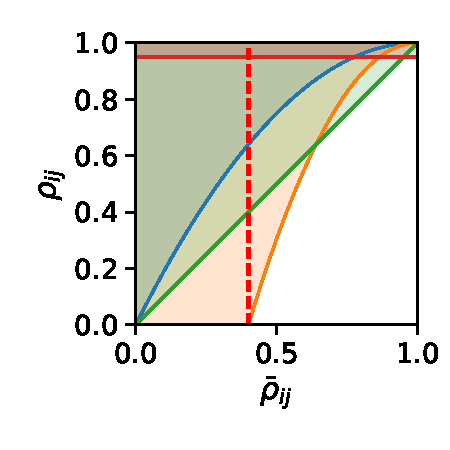
\includegraphics[scale=.6]{gfx/decision_funcs.pdf}
    \end{minipage}
    \hspace{-2.8em}
    \begin{minipage}{.3\textwidth}
    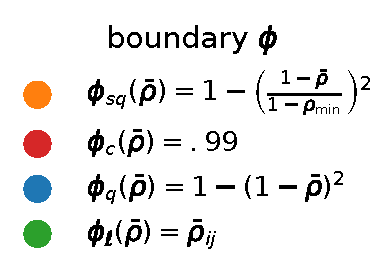
\includegraphics[scale=.6]{gfx/legend_1.pdf} \vfill
    \end{minipage}
	\caption[\ac{CV} redundancy heuristics]{Different decision functions
    used in the redundant control  variate removal. The weaker of any two control  variates is removed if
    the pair $(\bar\rho_{ij}, \rho_{ij})$ belongs to the shaded area of the considered function.
    The vertical dashed line indicates $\rho_{\min}$.\label{fig:decision}}
\end{figure}


Now, we discuss  the choice of the initial control  variates. We identify control  variate $k$ by
a tuple $({m}_k, \lambda_k)$ of a moment vector ${m}_k$
% \vw{vorher war $m_k$ ein vektor mit integern}
and a time-weighting
parameter $\lambda_k$.
% \vw{refer to equation?}
That is, we use $w(t)=e^{\lambda_k(T-t)}$ and $f(x)=x^{m_k}$ in \eqref{eq:poly_con}.
For a given set of parameters $L$, we use all moments up to some fixed order $n_{\max}$ (\autoref{line:init_covs}).
The ideal set of parameters $L$ is generally not known. 
For certain choices the correlation of the control  variates and the variable of interest is
higher then for others.
To illustrate this, consider the above example of the birth-death process.
Choosing $\lambda=-\delta$ leads to a control variate that has a correlation of $\pm 1$ with
$V$. Therefore, the ideal
choice of initial values for would be $L=\{-\delta\}$.
This, however, is generally not known.
Therefore, we sample a set of $\lambda$'s
from some fixed distribution $\pi_{\lambda}$ (\autoref{line:lambda_sample}).
\begin{figure}[htb]
    \centering
    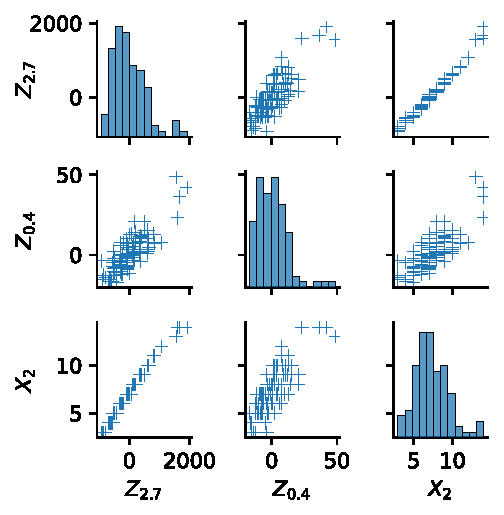
\includegraphics[scale=.65]{gfx/correlation.pdf}
    \hspace*{2em}
    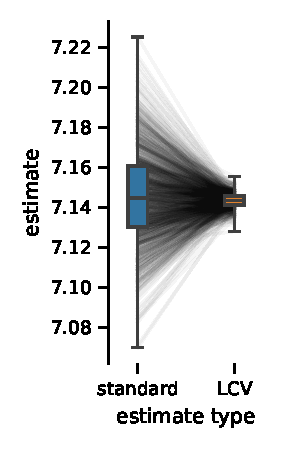
\includegraphics[scale=.65]{gfx/adjustment.pdf}
    \caption[\ac{CV} mean estimates v.\ std.\ mean estimates]{The effect of including \acp{CV} on the mean estimates $\hat{E}(X^M_2)$ in the dimerization case study. Parameters were ${\pi}_{\lambda}=N(0,1)$, ${n}_{\lambda}=30$, ${k}_{\min}=4$, $\phi(\bar\rho)=1-{(1 - \bar\rho)}^2$.}
\end{figure}


% \begin{itemize}
%     \item \textbf{Choice of control variates}
%     \item What needs to be logged.
%     \item Variance, Mean accumulation between runs
%     \item Choice of $\rho$ is done as the largest negative
%         eigenvalue of $Q$ \parencite{dowdy2018dynamic}.
% \end{itemize}

\section{Case Studies}\label{sec:cv:study}
We first define a criterion of \emph{efficiency} in order to estimate
whether the reduction in variance is worth the increased cost.
A natural baseline of a variance reduction is, that it is more efficient to pay for
the computational overhead of the reduction than to generate more samples to achieve a similar
reduction of variance.
Let $\sigma_Y^2$ be the variance of $Y$.
% https://statweb.stanford.edu/~owen/mc/Ch-var-basic.pdf
% Then the variance of the mean, based on $n$ iid.\ samples is $\sigma_Y^2/n$.
% If we let $c_0$ be the cost (i.e.\ CPU time) of a single simulation run, the overall cost to
% achieve this variance is $nc_0$.
% To achieve a variance $\tau^2$, $\sigma_Y^2/\tau^2$ samples are necessary at a cost of
% $c_0\sigma_Y^2/\tau^2$. We can analogously argue for the \ac{cv} estimate where the
% cost of a single iteration is $c_1$.
The \emph{efficiency} of the method is the ratio of the necessary
cost to achieve a similar reduction with the \ac{CV} estimate $Y_{\text{CV}}$ compared to
the standard estimate $Y$~\parencite{l1994efficiency}, i.e.
\begin{equation}\label{eq:efficiency}
E=\frac{c_0\sigma_Y^2}{c_1\sigma^2_{Y_{\text{CV}}}}\,.
\end{equation}
This is the ratio between \emph{slowdown} $c_0/c_1$ and variance reduction $\sigma_{Y}^2 / \sigma_{Y_{\text{CV}}}^2$.
That ratio $c_0/c_1$ depends heavily on both the specific implementation and the technical setup.
The cost increase is  mainly due to the computation of the integrals in \eqref{eq:simpl_exp}.
But the repeated checking of control  variates for efficiency also increases the cost.
The accumulation over the trajectory directly increases the cost of a single simulation
which is the critical part of the estimation.
To estimate the base-line cost $c_0$, $2000$ estimations were performed without
considering any control variates.

The simulation is implemented in the Rust programming language\marginpar{\url{www.rust-lang.org}}.
The model description is parsed from a high level specification. 
Rate functions are compiled to stack programs for fast evaluation.
Code is made available online \parencite{cme-simulation-github}.

We consider four non-trivial case studies. Three models exhibit complex multi-modal behaviour.
We now describe the models and the estimated quantities in detail.

The first model\graffito{This model appeared earlier as \autoref{model:dim} on page~\pageref{model:dim}.} is a simple dimerization on a countably infinite state-space.
\begin{model}[Dimerization]\label{model:dim2}
We first examine a simple dimerization model on an unbounded state-space.
	\[\varnothing\xrightarrow{10}M\,,\quad 2M\xrightarrow{0.1}D\]
with initial condition $X_0^M=0$.
\end{model}
Despite the models simplicity, the moment equations are not closed for this system
due to the second reaction which is non-linear.
Therefore a direct analysis of the expected value would require a closure.
For this model we will estimate $\E{X^M_2}$.

The following two models are bimodal, i.e.\ they each posses two stable regimes
among which they can switch stochastically.
For both models we choose the initial conditions such that the process
will move towards either attracting region with equal probability.
% This complex behaviour makes estimation particularly interesting, since
\begin{model}[Distributive Modification]\label{model:dm}
The distributive modification model was introduced in \parencite{cardelli2012cell}.
It consists of the reactions
\begin{gather*}
	X + Y \xrightarrow{\num{.001}} B + Y\,,\quad
	B + Y \xrightarrow{\num{.001}} 2 Y\\
	Y + X \xrightarrow{\num{.001}} B + X\,,\quad
	B + X \xrightarrow{\num{.001}} 2 X
\end{gather*}
with initial conditions $X^X_0=X^Y_0=X^B_0=100$.
\end{model}

% \begin{model}[Processive Modification]
% \parencite{cardelli2012cell}
% \begin{center}
% \begin{tabular}{c@{\hskip 1.5em}c@{\hskip 1.5em}c@{\hskip 1.5em}c}
%     $X + Y \xrightarrow{0.01} B + Y \,,$&
%     $X \xrightarrow{0.01} B       \,,  $&
%     $Y + X \xrightarrow{0.01} C + X\,, $&
%     $Y \xrightarrow{0.01} C \,,$\\

%     \rule{0pt}{4ex}$B + Y \xrightarrow{0.01} 2 Y \,,  $ &
%     $B \xrightarrow{0.01} Y    \,,   $&
%     $C + X \xrightarrow{0.01} 2 X\,, $ &
%     $C \xrightarrow{0.01} X       $
% \end{tabular}
% \end{center}
% with initial conditions $X_X(0)=10,\!000$ and all other species at $0$.
% \end{model}

\begin{model}[Exclusive Switch]\label{model:es}
	The exclusive switch model consists of \num{5} species, \num{3} of which are typically binary (activity states of the genes) \parencite{loinger2007stochastic}.
\begin{gather*}
	D + P_1 \xrightarrow{\beta} D.P_1\,,\quad
	D.P1 \xrightarrow{\gamma_1} D + P_1  \,,\\
	D + P_2 \xrightarrow{\beta} D.P_2 \,,\quad
	D.P2 \xrightarrow{\gamma_2} D + P_2 \,,\\
	D.P_1 \xrightarrow{\rho_1} D.P_1 + P_1\,, \quad
    D.P_2 \xrightarrow{\rho_2} D.P_2 + P_2\,,\\
	D \xrightarrow{\rho_1} D + P_1\,,\quad
	D \xrightarrow{\rho_2} D + P_2\,,  \quad
	P_1 \xrightarrow{\lambda}\varnothing  \,,\quad
    P_2\xrightarrow{\lambda} \varnothing
\end{gather*}
with initial conditions 
	\[X^D_0=1 \text{ and } X^{D.P1}_0=X^{D.{P_2}}_0=X^{P_1}_0=X^{P_2}_0=0\,.\]
\end{model}

We evaluate the influence of algorithm parameters, choices of distributions
to sample $\lambda$ from, and the influence of the sample size on the efficiency of
the proposed method.
Note that the implementation does not simplify the constraint representations
or the state space according to stoichiometric invariants or limited
state spaces.
\autoref{model:dm}, for example has the invariant 
\[
	X^X_t+X^Y_t+X^B_t=\text{const.}$, $\forall t\geq 0\,,
\]
which could be used to reduce the state-space dimensionality to two.
In \autoref{model:es} the invariant 
\[
	\forall t\geq 0.X^D_t,X^{D.{P_1}}_t,X^{D.{P_2}}_t\in\{0,1\}
\]
could be used to optimize the algorithm by eliminating redundant moments, e.g.\ $\expSym({(X^D)}^2)=\E{X^D}$.
Such an optimization would further increase the efficiency of the algorithm.




We first turn to the choice of the $\lambda$ sampling distribution. Here we
consider two choices:
\begin{enumerate}
    \item a standard normal distribution $N(0,1)$,
    \item a uniform distribution on $[-5,5]$.
\end{enumerate}
We deterministically include $\lambda=0$ in the constraint set, as this parameter
corresponds to a uniform weighting function.
We performed estimations on the case studies using different valuations of the
algorithm parameters of the minimum threshold $k_{\min}$ and
the number of $\lambda$-samples $n_{\lambda}$.
We used samples size $n=\num{10000}$ and checked the control  variates every $d=100$ iterations
for the defined criteria.
For each valuation \num{1000} estimations were performed.
In \autoref{fig:efficiencies_prior}, we summarize the efficiencies
for the arising parameter combinations on the three case studies.
Most strikingly, we can note that the efficiency was consistently larger than one in
all cases.
Generally, the normal sampling distribution out-performed the 
alternative uniform distribution, except in case of the dimerization.
The reason for this becomes apparent, when examining \autoref{fig:bdim}:
In case of the dimerization model the most efficient constraints are found for
$\lambda\approx -3$, while in case of the distributive modification they are located
 just above $0$ (we observe a similar pattern for the exclusive switch case study).
Therefore the sampling of efficient $\lambda$ values is more likely
using a uniform distribution for the dimerization case study, than it is for the others.
Given that larger absolute values for $\lambda$ seem unreasonable due 
their exponential influence on the weighting function and the problem of fixing
a suitable interval for a uniform sampling scheme, the choice of a standard normal
distribution for $\pi_{\lambda}$ seems superior.
\begin{figure}[htb]
    \centering
    \begin{minipage}{0.6\textwidth}
        \vfill
    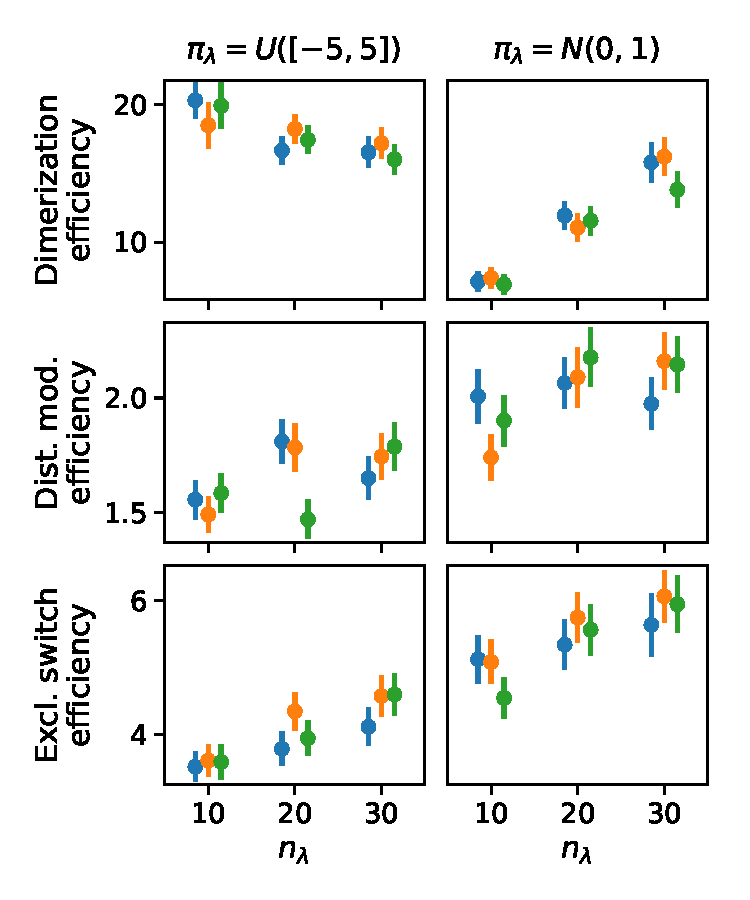
\includegraphics[scale=.5]{gfx/efficiency_priors.pdf}
    \vfill
    \end{minipage}
    \begin{minipage}{0.2\textwidth}
        \vfill
    
\includegraphics[scale=.7]{gfx/legend.pdf}
        \vfill
    \end{minipage}
	\caption[Estimates for varying ${n}_{\lambda}$ and ${k}_{\min}$]{The efficiencies for different valuations of ${n}_{\lambda}$ and ${k}_{\min} $
	and choices of ${\pi}_{\lambda}$. The sample size was $n=\num{10000}$ in all cases
    with $d=100$.
    The bars give the bootstrapped ($1000$ iterations) standard deviations.\label{fig:efficiencies_prior}}
\end{figure}

In \autoref{fig:efficiencies_order} we compare efficiencies for
different maximum orders of constraints $n_{\max}$.
This comparison is performed for different choices
of the redundancy rule and initial $\lambda$ sample sizes $n_{\lambda}$.
Again, for each parameter valuation \num{1000} estimations were performed.
With respect to the maximum constraints order $n_{\max}$ we see a clear
tendency, that the inclusion of second order
constraints lessens the efficiency of the method.
In case of a constant redundancy threshold it even dips below break-even
for the distributive modification case study.
This is not surprising, since the inclusion of second order moments
increases the number of initial constraints quadratically
and the incurred cost, especially of the first iterations,
lessens efficiency.
\begin{figure}[htb]
    \centering    
    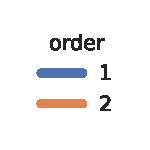
\includegraphics[scale=.55]{gfx/legend_orders.pdf}\\
    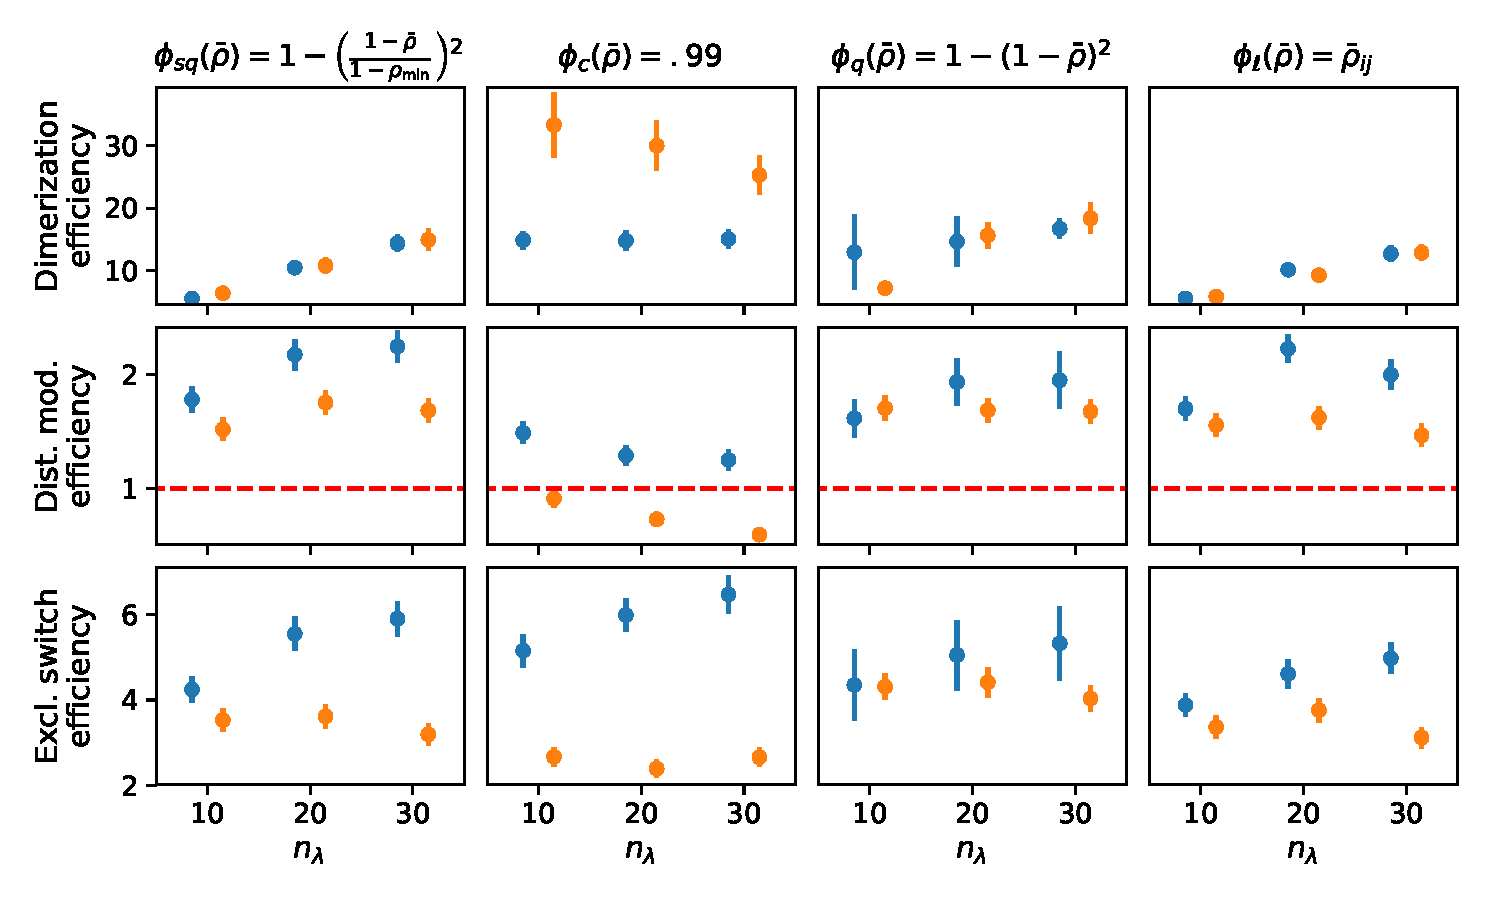
\includegraphics[scale=.4]{gfx/efficiency_ord1.pdf}
	\caption[Estimates for varying redundancy heuristics
	and moment orders]{The efficiency for different redundancy policies $\phi$ and maximal 
	moment orders $n_{\max}$. The sample size was $n=\num{10000}$ in all cases
    with $d=100$. Furthermore, $k_{\min}=3$, $\pi_\lambda=N(0,1)$, and $n_{\max}=1$.
    The bars give the 
    bootstrapped ($1000$ iterations) standard deviations.\label{fig:efficiencies_order}}
\end{figure}
\begin{figure}[htb]
    \centering    
    
\includegraphics[scale=.55]{gfx/legend.pdf}\\
    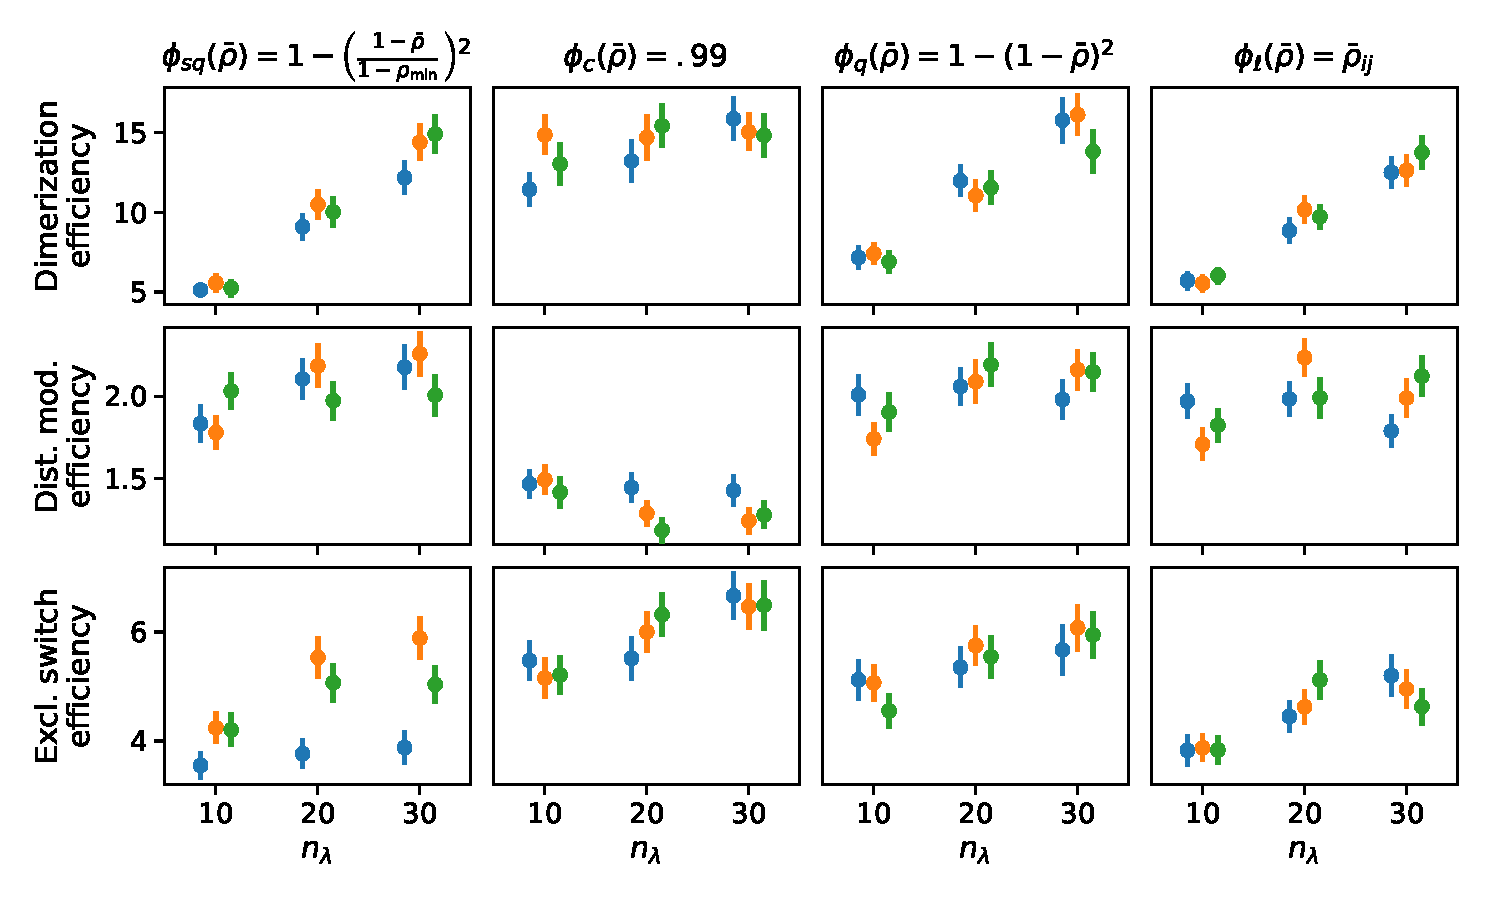
\includegraphics[scale=.4]{gfx/efficiency_pminfrac.pdf}
	\caption[Varying redundancy heuristics and $k_{\min}$]{The empirical efficiencies for different $n_\lambda$ and $k_{\min}$.
	On the considered case studies. The sample size was $n=\num{10000}$ in all cases
    with $d=100$.
	$\num{1000}$ estimations were performed for each case.
    The bars give the 
	bootstrapped (\num{1000} iterations) standard deviations.
    The break-even $E=1$ is marked by the dotted red line.\label{fig:efficiencies_alg_params}}
\end{figure}



\autoref{fig:trade_off} depicts the trade-off between the variance reduction $\sigma_0^2/\sigma_1^2$
versus the cost ratio $c_0/c_1$. Comparing the redundancy criterion based on a constant threshold
$\phi_c$ to the others,
we observe both a larger variance reduction and an increased cost. This is due to the fact, that
more control  variates are included throughout the simulations (\autoref{tab:eff1}, \autoref{tab:eff2}, \autoref{tab:eff3}). Depending on the sample distribution $\pi_{\lambda}$
and the case study, this permissive strategy may pay off. In case of the dimerization, for example,
it pays off, while in case of the distributive modification it leads to a lower efficiency ratio.
In the latter case the model is more complex, and therefore the set of initial
control  variates is larger. With a more permissive redundancy strategy, more control  variates are kept
(ca.\ $10$ when using $\phi_c$ vs.\ ca.\ \numrange{2}{3} for the others).
The other redundancy boundaries move the results further in the direction of less variance reduction
while keeping the cost increase low.
On the opposite end is the linear $\phi_{\ell}$.
The quadratic versions $\phi_{q}$ and $\phi_{\mathit{sq}}$ can be found in the middle of this spectrum.
\begin{figure}[tb]
    \centering
    \hfill
    \begin{minipage}{\textwidth}
    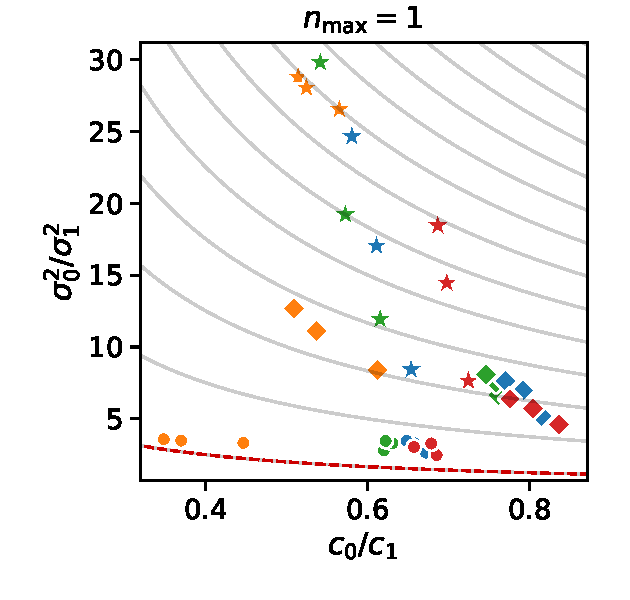
\includegraphics[scale=.5]{gfx/eff_landscape_order1.pdf}
    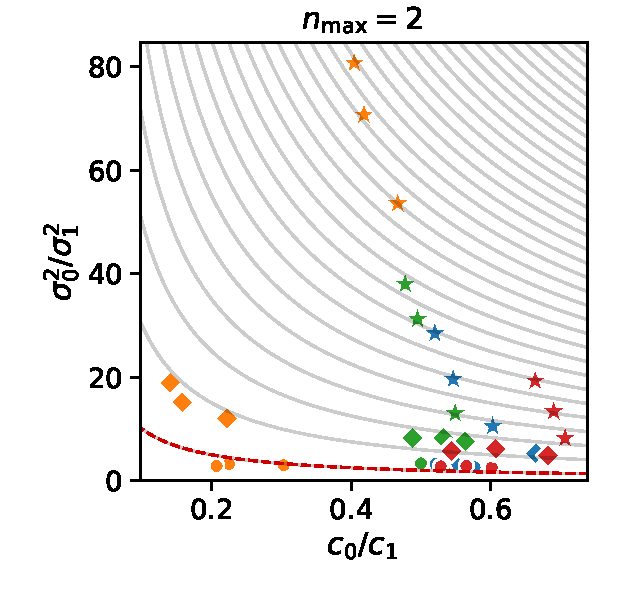
\includegraphics[scale=.5]{gfx/eff_landscape_order2.pdf}
    \end{minipage}
    \hfill
    \begin{minipage}{.4\textwidth}
	    \vfill
    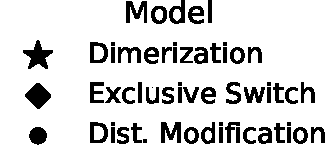
\includegraphics[scale=.5]{gfx/legend_models.pdf}
	    \vfill
    \end{minipage}
    \begin{minipage}{.4\textwidth}
	    \vfill
    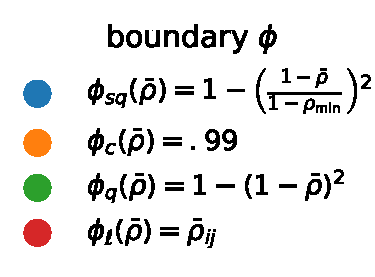
\includegraphics[scale=.5]{gfx/legend_phi.pdf}
	    \vfill
    \end{minipage}
    \hfill
    \caption[Cost \& variance reduction trade-off]{A visualisation of the trade-off between variance reduction $\sigma_0^2/\sigma_1^2$
    and cost ratio $c_0/c_1$. Isolines for efficiencies are given in grey. The break-even
    is marked by the dashed red line.
    Markers of the same kind differ in $n_{\lambda}$ and shift with increasing value
    upwards in variance reduction and lower in $c_0/c_1$, i.e.\ the shift is to the left and upwards
    with increasing $n_{\lambda}$.
	The sample size was $n=\num{10000}$ in all cases
    with $d=100$. Furthermore, $k_{\min}=3$ and $\pi_\lambda=N(0,1)$.}
    \label{fig:trade_off}
\end{figure}

We also observe, that an increase of $n_{\lambda}$ is particularly beneficial, if
the sampling distribution $\pi_{\lambda}$ does not capture the parameter region of
the highest correlations well.
This can be seen for the Dimerization case study, where the variance reduction increases
strongly with increasing sample size (\autoref{fig:efficiencies_alg_params}, \autoref{tab:eff1}, \autoref{tab:eff2}, \autoref{tab:eff3}).
Since $\pi_{\lambda}=N(0,1)$, more samples are needed to sample efficient $\lambda$-values (cf.\ \autoref{fig:bdim}).

In \autoref{fig:efficiencies_alg_params} we give detailed information on the influence of
algorithm parameters $k_{\min}$, the number of initial $\lambda$ values, and
different redundancy rules.
The $\lambda$ sampling distribution $\pi_{\lambda}$ is a standard normal.

Finally, we discuss the effect of the sample size $n$ on the efficiency $E$. In \autoref{fig:sample_sizes}
we give both the efficiencies and the slowdown for different sample sizes.
As a redundancy rule we used the unscaled quadratic function, $30$ initial values of $\lambda$,
and $k_{\min}=3$. With increasing sample size, the efficiency usually approaches an upper limit.
This is due to the fact that most control  variates are dropped early on and
the control  variates often remain the same for the rest of the simulations.
If we assume there are no helpful control  variates in the initial set
and all would be removed at iteration $100$, the efficiency would converge to $1$
for $n\to \infty$.
\begin{figure}[htb]
	\myfloatalign
	\subfloat[Efficiency v.\ sample size]
	{\label{fig:sample_sizes:eff}
	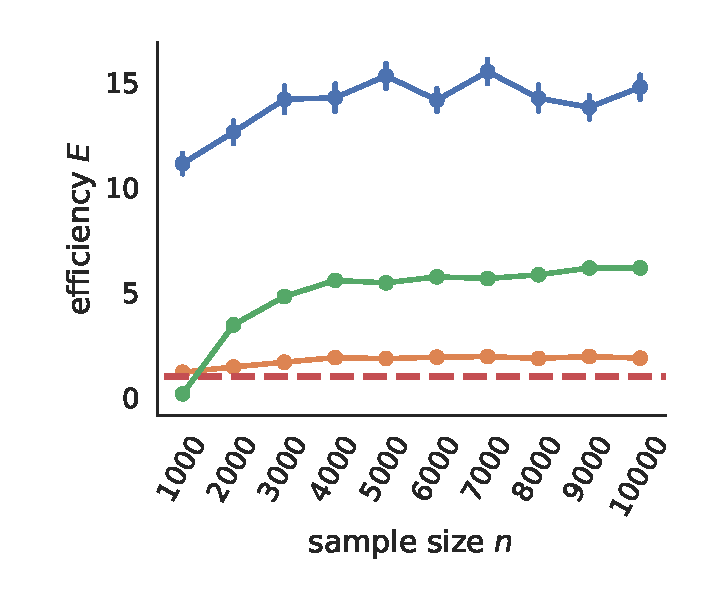
\includegraphics[scale=.38]{gfx/sample_size_efficiency.pdf}}\quad
	\subfloat[Slowdown v.\ sample size]
	{\label{fig:sample_sizes:slowdown}
	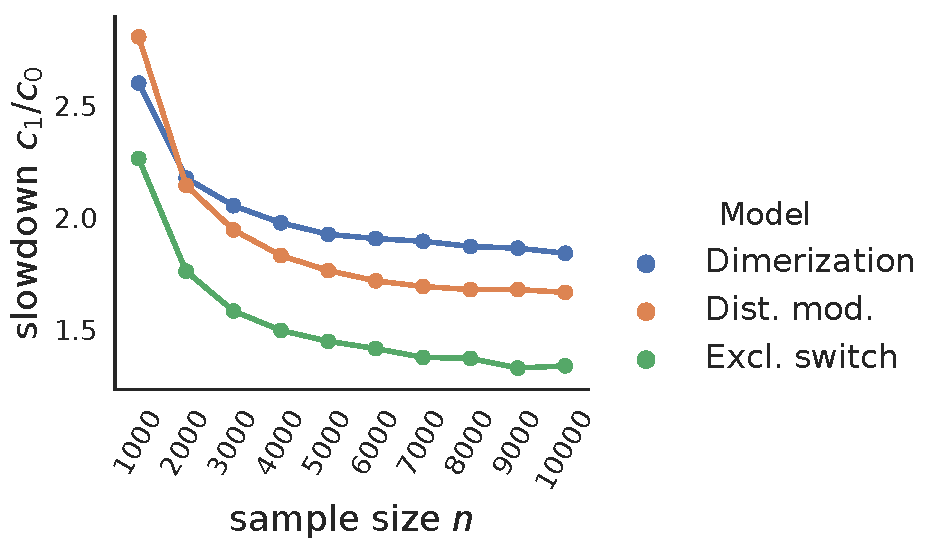
\includegraphics[scale=.38]{gfx/sample_size_slowdown.pdf}}
	\caption[Effect of sample size on control variate performance]{
    The effect of sample size on the efficiency $E$ and slowdown in the different case studies.
    The break-even $E=1$ is marked by the dashed red line.
    The cost increase due to the variance reduction over different sample sizes.}
    \label{fig:sample_sizes}
\end{figure}

%%%%%%%%%%%%%%%%%%%%%%%%%%%%%%%%%%%%%%%%%%%%%%%%%%
% Festschrift material %%%%%%%%%%%%%%%%%%%%%%%%%%%
%%%%%%%%%%%%%%%%%%%%%%%%%%%%%%%%%%%%%%%%%%%%%%%%%%
\section{Resampling Algorithm}\label{sec:splitting}
In previous work \parencite{backenkohler2019control}, we have proposed an algorithm that learns a set of
control variates through refinement of an initial set.
This initial set of control variates is based on samples of the time-weighting $\lambda$.
Each control variate is then checked for effectiveness in isolation.
Furthermore the set is refined by considering variable pairwise to determine redundancies.

In this work, we improve on the initial selection of control variates.
The initial set of control variates is build using a splitting approach akin to sequential Monte Carlo methods:
Over multiple rounds, new control variates are samples based on performance in prior rounds.
That way, a set of variates is build up.
This set is then refined in a greedy manner, taking into account the correlation between variates.
This algorithm has the main benefit of needing less sensitive to user input.
In particular, no heuristic redundancy threshold has to be fixed, making this approach more flexible.

As we have seen in the previous section, effective control variates have a high correlation
with the target random variable.
In the case of a single variate, the variance reduction is directly proportional to $1-\rho^2$, where
$\rho$ is the correlation.
In our case, infinitely many choices of $Z$ are available.
Our goal is to choose a subset that
satisfies two objectives:
Firstly, every selected control variate should reduce the estimator's variance.
Secondly, the subset should not be too large, i.e.  we want to avoid redundancies to achieve 
 a good  overall computational efficiency of the variance reduction.


%Accordingly, we define an \emph{efficiency} value to estimate
%whether the reduction in variance is compensating for the associated cost increase.
%A natural baseline of any variance reduction is that it outweighs its associated additional costs.
%Let $\sigma_Y^2$ be the variance of $Y$.
% https://statweb.stanford.edu/~owen/mc/Ch-var-basic.pdf
% Then the variance of the mean, based on $n$ iid.\ samples is $\sigma_Y^2/n$.
% If we let $c_0$ be the cost (i.e.\ CPU time) of a single simulation run, the overall cost to
% achieve this variance is $nc_0$.
% To achieve a variance $\tau^2$, $\sigma_Y^2/\tau^2$ samples are necessary at a cost of
% $c_0\sigma_Y^2/\tau^2$. We can analogously argue for the CV estimate where the
% cost of a single iteration is $c_1$.
%The \emph{efficiency} of the method is the ratio of the necessary
%cost to achieve a similar reduction with the CV estimate $Y_{\text{CV}}$ compared to
%the standard estimate $Y$~\parencite{l1994efficiency,mcbook}, i.e.
%\begin{equation}
%E=\frac{c_0\sigma_Y^2}{c_1\sigma^2_{Y_{\text{CV}}}}\,.
%\end{equation}
%The cost ratio $c_0/c_1$ depends on both the specific implementation and the technical setup.
%The cost increase is  mainly due to the computation of the integrals in \eqref{eq:dis_int}.
%The accumulation over the trajectory directly increases the cost of a single simulation,
%which is the critical part of the estimation.

If the computation of a variate does not adequately compensate for its computation
with variance reduction, we do not want to include it.
Balancing both objectives is challenging because control variates often correlate with each other.
Such correlations expose redundancy between different variates.
This also becomes clear, when considering that the overall variance reduction  depends on
the coefficient of multiple correlation.
% \vw{is multiple the right word here? }

Here we follow a resampling paradigm:
We start by building up a set of candidates using a particle splitting approach.
After each splitting step, we generate a small number of \ac{SSA} samples to estimate correlations.
Promising candidates are chosen based on the \emph{improvement} they provide and their time-weighting parameter $\lambda$ is resampled (see \autoref{fig:resampling}).
The main benefit of this bottom-up approach is its lower dependence on the initial sampling distribution of $\lambda$.
Moreover, the procedure spends less time evaluating unpromising candidates.
After   generating a set of control variates, the overall covariance matrix is estimated using stochastic simulations.
Using this information, we construct an efficient subset using a greedy scheme, taking into account the redundancies between control variates.
We discuss \autoref{alg:splitting:lcv} in more detail below.

\begin{figure}
    \centering
    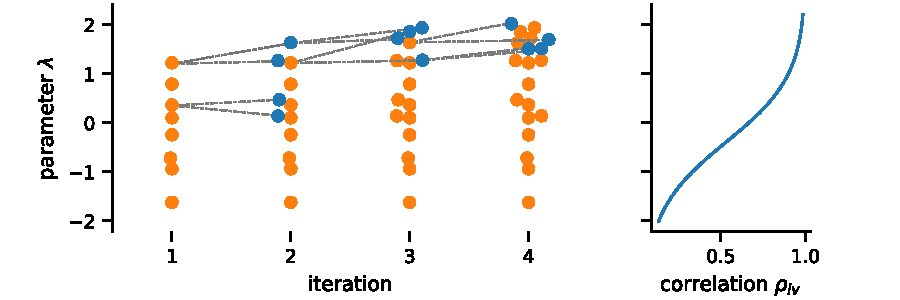
\includegraphics[scale=0.65]{gfx/resampling.pdf}
    \caption[Resampling algorithm]{An illustration of the resampling procedure for the time-weighting parameter $\lambda$ using \autoref{model:dm}. Areas giving higher correlations are resampled through multiple rounds. The newly sampled values are given in blue. In each round only the new candidates are evaluated.}
    \label{fig:resampling}
\end{figure}


\begin{algorithm}[ht]
\SetKwInOut{Input}{input}
\SetKwInOut{Output}{output}
\Input{$n, d, n_{\max}, n_{\lambda}, n_{c}, n_s, n_r$}
\Output{estimate using linear control variates}
  $L\leftarrow\{\lambda_i\sim \pi_\lambda \mid 1\leq i< n_{\lambda} \} \cup \{ 0 \}$\label{line:resampling:lambda_sample}\tcc*[r]{initialization}
  $P \leftarrow \{ ({m}, \lambda) | 1\leq\lvert {m} \rvert \leq n_{\max}, \lambda\in L\}$\label{line:resampling:init_covs}\;
  $P_{\text{all}} = \emptyset$
    \For{$i=1,\dots,n_r$\label{line:resampling:main_loop} \tcc*[r]{resampling}}{
        $(\hat{\Sigma},\hat{V}, \hat{Z}) \leftarrow \text{SSA}_{\text{CV}}(\pi_0,T,P,d)$\;

     $P_{\text{all}}\leftarrow P_{\text{all}}\cup P$\;
     $I_{\text{cands}}\leftarrow \{ k\sim \hat\gamma_{kv}/ \sum_{\ell}\hat{\gamma}_{\ell v} \mid 1\leq k \leq |P_{\text{all}}|, j=1,\dots,n_c\}$\label{line:resampling:resample}\;
     $P\leftarrow \bigcup_{k\in I_{\text{cands}}}\bigcup_{l=1}^{n_s}
     \{(m_k, \lambda_k') \mid \lambda_k'\sim N(\lambda_k, 0.5)\}$\label{line:resampling:end_resampling}\;
  	}
    $(\hat{\Sigma},\hat{V}, \hat{Z}) \leftarrow {\text{SSA}}_{\text{CV}}(\pi_0,T,P_{\text{all}},5d)$\label{line:resampling:search_loop}\tcc*[r]{covariance}
     $P^*=\emptyset$\;
     \While{$\exists i:
        (m_i, \lambda_i)\in P_{\text{all}}\setminus P^*\land$\\
        \hspace{4em}$\hat{\gamma}_{iv} \prod_{j=1;(m_j, \lambda_j)\notin P^*}^{\left|P_{\text{all}}\right|}
        \hat{\gamma}_{ij}^{-1}
        >\epsilon$\tcc*[r]{selection}\label{line:resampling:selection_loop}}{
        $k \leftarrow \argmax_i \hat{\gamma}_{iv}
        \prod_{j=1;(m_j, \lambda_j)\notin P^*}^{\left|P_{\text{all}}\right|}
        \hat{\gamma}_{ij}^{-1}$\label{line:resampling:selection}\;
        $P^*\leftarrow P^* \cup
            \{(m_k,\lambda_k)\}$\;
    }
    $(\hat{\Sigma},\hat{V}, \hat{Z}) \leftarrow \text{SSA}_{\text{CV}}(\pi_0,T,P^*,n)$\tcc*[r]{estimation}\label{line:resampling:sim}
    \Return $\hat{V} - {(\hat{\Sigma}_{{Z}}^{-1}\hat\Sigma_{{Z}V})}^{\top}\hat{{Z}}$\label{line:resampling:compute_lcv}
    \caption{\label{alg:splitting:lcv}Estimate the mean of species $i$ at time $T$}
\end{algorithm}

\paragraph{Initialization} A tuple $({m}_k, \lambda_k)$ of a moment vector ${m}_k$ and a time-weighting parameter $\lambda_k$
uniquely identifies a control variate $k$.
The algorithm starts out with an initial small set of control variates.
That is, we use $w(t)=e^{\lambda_kt}$ and $f(x)=x^{m_k}$ in \eqref{eq:poly_con}.
For a given set of time-weighting parameters $L$, we use all moments up to some fixed order $n_{\max}$ (\autoref{line:resampling:init_covs}).
For a fixed moment vector $m_k$ the time-weighting parameter $\lambda_k$ can lead to vastly different correlations $\rho_{kv}$ with the quantity of interest.
The best choices of $\lambda$ are usually not known beforehand.
Therefore, we sample an initial set of $\lambda$'s
from a fixed distribution $\pi_{\lambda}$ (\autoref{line:resampling:lambda_sample}).
Here, we use a standard normal distribution because its mean is the neutral weighting of $\lambda=0$ and extreme values are unlikely.

\paragraph{Resampling} Promising candidates are chosen from all control variates based on the estimated \emph{improvement ratio} they
provide, i.e.\ 
\begin{equation}
\hat{\gamma}_{kv} = ({1 - \hat{\rho}_{kv}^2})^{-1}
\end{equation}
following \eqref{eq:lcv_norm_varred}.
Specifically, control variate $k$ is chosen with probability proportional to
${\hat{\gamma}}_{kv}$ (\autoref{line:resampling:resample}).
The covariances of (only) the new variates are roughly estimated using very few (e.g., $d= 10$) \ac{SSA} samples. 
For the selected variates $I_{\text{cands}}$, the time-weighting parameter is resampled using a step distribution.
There is some freedom in the specifics of this resampling procedure.
In particular, the number of splits $n_c$ and descendants $n_s$ for each candidate control the number of additional candidates.
The algorithm performs $n_r$ rounds of resampling.
\autoref{fig:resampling} illustrates this part of the algorithm.

\paragraph{Covariance Estimation} After sampling a set of candidates this way, we need to select the most promising ones.
For this, we are interested in covariances between all control variates, as well.
Since the resampling does not provide us with such estimates, we evaluate all candidates together for a fixed number of simulations (\autoref{line:resampling:search_loop}).

\paragraph{Selection} The selection part of the algorithm (\autoref{line:resampling:selection_loop}) proceeds in a greedy fashion wrt.\ the potential estimated improvement $\hat{\gamma}_{iv}$ given by any variate.
However, covariates often have high mutual correlations.
For example, $Z_{\lambda}$ and $Z_{\lambda+\epsilon}$ for a small $\epsilon$ are typically highly correlated --- often more with each other than with the objective.
We want to avoid this unnecessary computational overhead from computing nearly redundant information and numerical problems due to the covariance matrix inversion (see \eqref{eq:lcv_asym}).
As a solution, we normalize the estimated improvement vector $(\hat{\gamma}_{iv})_i$ by
the product of the fractions of explained variances by the already selected covariates.
Therefore we choose the most promising candidate given a selection $P^{*}$ as
\begin{equation}
\argmax_{1\leq i \leq \left|P_{\text{all}}\right|}
\hat{\gamma}_{iv}
    \prod_{\substack{1\leq j\leq {\left|P_{\text{all}}\right|}\\(m_j, \lambda_j)\notin P^*}}
    \hat{\gamma}_{ij}^{-1}
\end{equation}
in \autoref{line:resampling:selection}.
This selection is done, until some lower threshold $\epsilon$ is reached (\autoref{line:resampling:selection_loop}).

\paragraph{Estimation} Finally, we simulate the model $n$ times (\autoref{line:resampling:sim}).
The resulting information enables an LCV estimation (\autoref{line:resampling:compute_lcv}).


We applied the presented algorithm for an estimation using $n=\num{10000}$ simulations.
Initially $n_{\lambda}=10$ samples for the time-weighting parameter were drawn from a standard normal distribution ($\pi_{\lambda} = N(0,1)$).
Constraints corresponding to each first-order moment, i.e.\ the process' expectations were generated ($n_{\max}=1$).
The covariance estimation during resampling used $d=10$ samples.

We evaluated the algorithm both with and without resampling for these first two case studies.
The algorithm without resampling  leaves out lines~\ref{line:resampling:main_loop}--\ref{line:resampling:end_resampling} from \autoref{alg:splitting:lcv}.
The evaluation without resampling provides a good point of comparison to our previous heuristics performance on these cases.
In the case of dimerization we observe a variance reduction of $\approx 27.67$ compared to a best case reduction of $\approx 28.75$ in our previous work.
This close performance however has to balance very different slowdown factors: With our new heuristic the slowdown is a factor of $\approx 1.34$ while in the previous case it was $\approx 1.95$.
Therefore the new method clearly outperforms in terms of efficiency ($\approx 20.5$ (new) versus $\approx 14.86$ (old)).
This is mainly due to the higher number of covariates used by the simple threshold heuristic.
In contrast the new method takes into account redundancies between covariances while still retaining good performance.
This becomes apparent when comparing the average number of used variates ($\approx 3.34$ (old) versus $\approx 1.98$ (new)).

The variance reduction factor for the distributive modification model is similar at $\approx 2.63$ (old) versus $\approx 2.66$ (new).
Noticeably, the new method uses on average fewer CVs ($\approx 2.74$) than the previous heuristic with the best efficiency ($\approx 3.23$).
The overall efficiency of the new algorithm with $1.72$ is slightly lower than the previous best value of $1.77$, due to a higher slowdown.
It is however important to note, that the trade-off differs significantly between different  heuristics used in the previous algorithm.
Furthermore, the lower average number of control variates would reduce the slowdown factor further, if more trajectories are generated.
% \paragraph{Filtering algorithm findings}
% \begin{itemize}
% \item results compared to prev work
%     \begin{itemize}
%     %     \item better for dimerization than previous work $(0.965224 1.945588 14.859417 3.338501)$
%     %     28.75546353807221 var red
%     %     1.945588 slodown
%     %      14.859417 efficiency (constant red)
%     %     versus 
%     % (1.3498338896993884, 27.6717070777087, 20.50008322421899)
%()
%     \item comparable for dist. mod (1.5462838232319676, 2.6620853997091847, 1.7216020498390927)
%     0.619560 1.488483 1.770218 3.232575
%     2.628535380086216 varred
%     \item much fewer LCV
%     \item Higher variance for lower correlations? (check this)
% \end{itemize}
% \end{itemize}
\begin{figure}[htb]
    \centering
    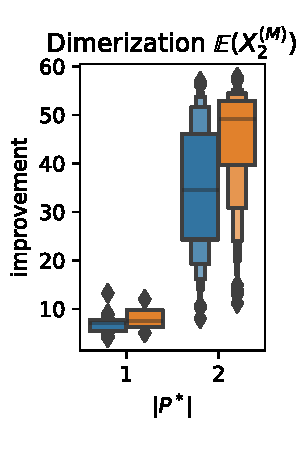
\includegraphics[scale=.65]{gfx/dim_improvement_numcv.pdf}
    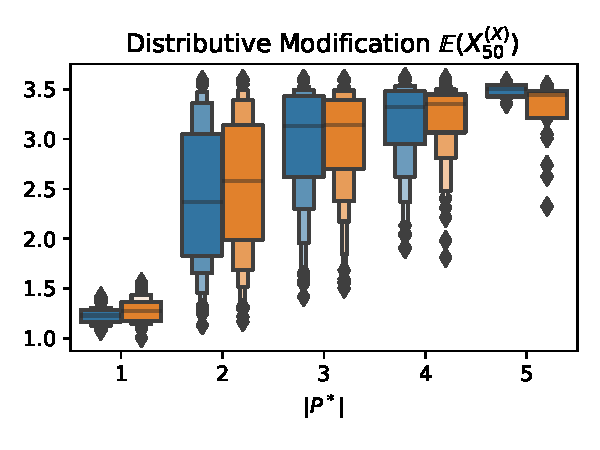
\includegraphics[scale=.65]{gfx/dm_improvement_numcv.pdf}
    
\includegraphics[scale=.65]{gfx/improvement_numcv_legend.pdf}
    \caption[Number of \ac{CV} v.\ variance reduction]{\label{fig:cv:refinement}The variance reduction factor $\sigma_{Y}^2 / \sigma_{Y_{LCV}}^2$ over different numbers of selected covariates with and without the resampling procedure.}
\end{figure}

In \autoref{fig:cv:refinement} we contrast the variance improvement ratio with and without the resampling algorithm. For the dimerization model, we see a clear improvement of variance reduction.
This improvement is due to the fact that the strongest correlations are present for $\lambda \approx 2.5$ (cf.\ \autoref{fig:resampling}).
This region of the time-weighting parameter space is less likely to be sampled by the initial
samples from the standard normal distribution.
Therefore the resampling procedure is especially beneficial if the better parameters $\lambda$ are farther from the origin.
In case of the distributive modification case study, we see a slight improvement.
Here, the best parameters $\lambda$ are close to zero and thereby more likely to be sampled by a standard normal.
Still, the resampling improves covariate performance for the most frequent cases of 2--4 covariates being selected (the case of 5 covariates has only a few instances).
Note, that the additional cost incurred by the resampling procedure is comparatively small, because
at most 4 candidates are evaluated in each iteration.
% \paragraph{SMC findings}
% \begin{itemize}
%     % \item The resampling makes finding better $Z$ more likely
%     \item resampling incurs a lower additional cost than a larger initial $L$ (because $|L| n_S^{n_{\max}}$
%     \item less reliance on $\pi_{\lambda}$
%     \item Figure \ref{fig:cv:refinement} discussion
%     \begin{itemize}
%         \item consistent improvement
%         \item most prominent with dimerization, because high correlations farther away from zero
%         \item $|P^*|=5$ and dist. mod. are few examples
%     \end{itemize}
% \end{itemize}


Next, we turn to the estimation of probabilities.
In particular, we consider the event of a species being below a threshold $\ell$ at time $t$ (species $M$ for the dimerization and $X$ for the distributive modification).
In \autoref{fig:thresholds} we summarize the results of this study for varying levels $\ell$.
In both case studies we observe that control variates are efficient for probabilities not close to either zero or one.
In this case control variates are able to reduce the variance of the estimated probabilities whilst maintaining a beneficial reduction-slowdown trade-off.
This region is larger for the distributive modification model because of its bimodal behavior.
If the probability to be estimated is close to either one or zero, the event occurs too rarely or too often, respectively, to adequately explain variance using linear correlations.
We note, that the worst case efficiency is close to one.
This is due to the algorithm throwing out all covariate candidates leaving us with a standard estimation.
Only the initial covariate evaluation and resampling causes a slowdown, driving efficiency slightly below one.
Naturally this cost decreases with more samples $n$.

Control variates based on test functions restricted to intervals did not lead to an improvement (data not shown).

% \paragraph{Probability estimation}
% \begin{itemize}
%     \item LCV for Probabilities is most effective if probability is around .5
%     \begin{itemize}
%         \item Correlations can be more easily captured
%     \end{itemize}
%     \item LCV not effective for probs. close to 0 or 1
%     \item interval-based CVs do not perform better for threshold probabilities
% \end{itemize}
\begin{figure}[htb]
    \centering
    
\includegraphics[scale=0.65]{gfx/legend_thres.pdf}\\
    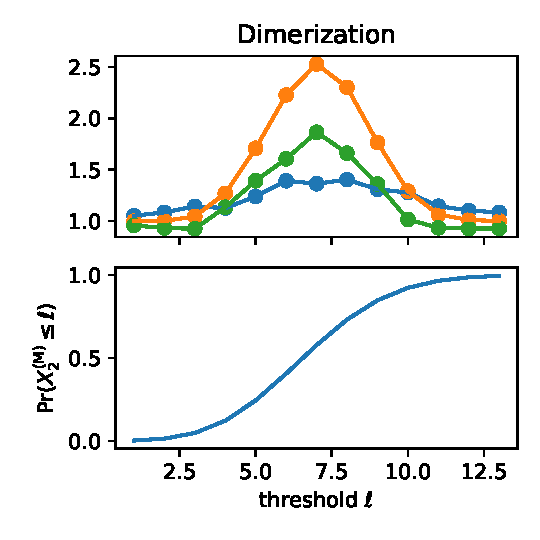
\includegraphics[width=.49\textwidth]{gfx/dim_thresholds.pdf}
    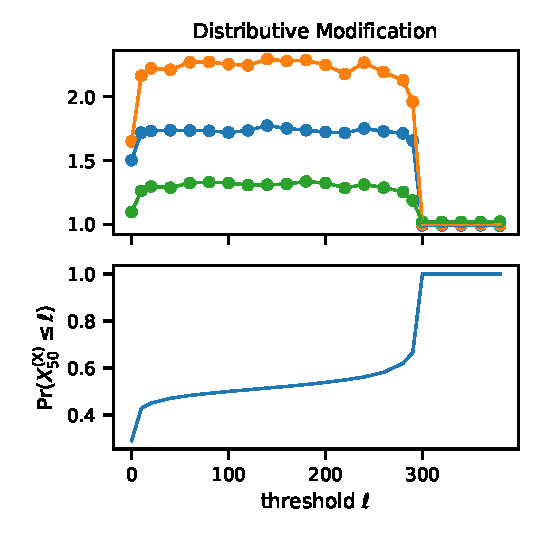
\includegraphics[width=.49\textwidth]{gfx/dm_threholds.pdf}
    \caption[\ac{CV} for probabililty estimation]{The methods efficiency for the estimation of threshold probabilities. For each threshold $\ell$ at least 200 estimations were performed.}
    \label{fig:thresholds}
\end{figure}


Finally, with the lac operon model we consider a larger case study. This model consists of 11 species and 25 partly non-linear reactions.
\begin{model}[Lac operon]\label{model:lac}This is a well-known model of genetic regulation with positive feedback \parencite{stamatakis2009comparison}. Its reactions are
 \begin{gather*}
 \varnothing \xrightleftharpoons[k_19]{k_1} \mathrm{M_R}\,, \quad
 \mathrm{M_R} \xrightarrow{k_2} \mathrm{M_R + R}\,,\quad
 2 \mathrm{R} \xrightleftharpoons[k_4]{k_3} \mathrm{R_2}\,,\\
 \mathrm{R_2 + O} \xrightleftharpoons[k_6]{k_5}\mathrm{ R_2O}\,,\quad
 \mathrm{2 I + R_2} \xrightleftharpoons[k_8]{k_7} \mathrm{I_2R_2}\,,\\
\mathrm{2I +R_2O} \xrightleftharpoons[k_{10}]{k_9} \mathrm{I_2R_2 + O}\,,\quad
\mathrm{O}\xrightarrow{k_{11}} \mathrm{O + M_Y}\,,\\
\mathrm{R_2O}\xrightarrow{k_{12}}\mathrm{R_2O+M_Y}\,,\quad
\mathrm{M_Y} \xrightarrow{k_{13}}\mathrm{M_Y + Y}\,,\\
\mathrm{Y + I_{{ex}}}\xrightleftharpoons[k_{15}]{k_{14}}\mathrm{YI_{{ex}}}\,,\quad
\mathrm{YI_{{ex}}}\xrightarrow{k_{16}}\mathrm{Y+I}\,,\quad
\mathrm{I_{{ex}}}\xrightleftharpoons[k_{18}]{k_{17}}\mathrm{I}\,,\\
\mathrm{M_Y}\xrightarrow{k_{20}}\varnothing\,,\quad
\mathrm{R}\xrightarrow{k_{21}}\varnothing\,,\quad
\mathrm{R_2}\xrightarrow{k_{22}}\varnothing\,,\quad
\mathrm{Y}\xrightarrow{k_{23}}\varnothing\,,\\
\mathrm{YI_{ex}}\xrightarrow{k_{24}}\mathrm{I}\,,\quad
\mathrm{I_2R_2}\xrightarrow{k_{25}}\mathrm{2I}\,.\quad
\end{gather*}
Initially, $X^{(\mathrm{O})}_0=1$ and $X^{(\mathrm{I_{{ex}}})}=\num{48177}$ while all other abundancies are zero.
The parameters are $
  k_1  = 0.111$,
 $ k_2  = 15.0$,
  $k_3  = 103.8$,
  $k_4  = \num{0.001}$,
  $k_5  = 1992.7$,
  $k_6  = 2.4$,
  $k_7 =k_9  = \num{1.293d-7}$
  $k_8  = 12$,
  $k_{10} = 9963.2$,
  $k_{11} = 0.5$,
  $k_{12} = 0.01$,
  $k_{13} = 30.0$,
  $k_{14} = 0.249$,
  $k_{15} = 0.1$,
  $k_{16} = \num{6.0d4}$,
  $k_{17} =k_{18} = 0.92$,
  $k_{19} = k_{20} = 0.462$,
  $k_{21}=k_{22}= k_{23} = k_{24} = k_{25} = 0.2$.
\end{model}
We estimate the abundancy of LacY after one time unit, i.e.\ $\expSym(X^{(Y)}_1)$.
It is encoded by Y and facilitates
the lactose import via reactions 14 and 16.
A typical simulation of the system up to time-horizon $T=1$ takes well above one minute of computational time.
Therefore we reduce the number of used trajectories to $n=1000$.
The other settings remain as above.

Despite the high dimensionality, we observe a good efficiency value of $E\approx 4.85$.
The slowdown caused by the method is approximately 1.98.
A big part of this slowdown is due to the initial search of covariates.
Initially 10 covariates are generated for each first order moment, i.e.\ each of the
11 species. The number of additionally resampled covariates is similar to previous case studies.
Thus the main cost of the initial resampling and selection is due to the first iteration of the
resampling loop and the simulation loop of the selection procedure.
This part naturally has still potential for optimization:
Not all known covariates need to be reconsidered at the selection stage.
Instead, unpromising candidates could be discarded prior to that stage.

Still, the high variance reduction by a factor of approx.\ ${9.64}^{-1}$ more than compensates for this increase in computational cost, leading to the good overall efficiency.
This shows that, even for more complex models, the method is applicable and can extremely beneficial for Monte Carlo estimation.
% \begin{itemize}
%     \item For larger models such as this one, the up front cost of evaluating too many initial $\lambda$s is exacerbated.
%     \item 11 species 25 reactions
%     \item expensive simulations
% \end{itemize}
% \paragraph{Scalability findings}
% \begin{itemize}
% \item Setting:\begin{itemize}
%     \item $\expSym(X^{(Y)}_1)$
%     \item \num{1000} SSA runs
%     \item settings as above
% \end{itemize}
%     \item System size (dimensionality in particular; 11 species) do not harm the algorithm; especially despite blowup of initial constraints
%     \item Implementation and setup may be worth it even more in such expensive-to-simulate models
%     \item Highlight how long one simulation takes
%     \item slowdown: 1.9845426838974896
%     \item variance reduction: 9.640543124900878
%     \item efficiency: 4.857815960888073)
% \end{itemize}

\section{Conclusion}\label{sec:cv:conclusion}
In the context of Monte Carlo simulation, variance reduction
techniques offer an elegant way of improving the performance without
introducing approximation errors in addition to the statistical uncertainty.
In this work we have shown that known constraints on the moment dynamics can be successfully
leveraged in simulation-based estimation of expected values.
The empirical results indicate that
the supplementing a standard \ac{SSA} estimation with moment information
can drastically reduce the estimators' variance.
This reduction is paid for by accumulating information on the trajectory
during simulation.
However, the reduction is able to compensate for this increase.
This means that for fixed costs, using   estimates with
  control variates is more beneficial than using estimates without control variates.


In particular, we improve an initial subset by selecting particularly effective variates and removing redundant variates.
By resampling the time-weighting parameter $\lambda$ we ensure that appropriate values  are
flexibly explored.
In the worst case, all variates are dropped and the performance approaches the standard \ac{SSA}.
In most cases, however, a suitable subset is found together with the corresponding choices of $\lambda$.

We  analyze the performance of the method when estimating event probabilities and not only average molecule counts. Our largest case study has 11 species and
24 reactions. %We achieve efficiencies of around \vw{say here what typical efficiencies are ; 2-4? Ist ja nicht viel ...}.

Another open question regarding this work is its performance when multiple
quantities instead of a single quantity are to be estimated. In such
a case, constraints would be particularly beneficial, if they lead
to improvements  as many estimation targets as possible.


In the future, we will further explore the algorithmic design space.
For example, the resampling distribution could be adjusted using decaying standard deviations.
Furthermore, we will look at different test functions weighting the state space more flexibly.
Different choices of $f$ and $w$ in \eqref{eq:poly_con} may improve 
efficiency further.
These choices become particularly interesting when moving from the estimation
of simple first order moments to more complex queries such as behavioural probabilities
of trajectories.
In such cases, one might even attempt to find efficient control variate functions
using machine learning methods.

Another worthwhile direction is the combination of \ac{CV} with other Monte Carlo techniques.
In particular, importance sampling might benefit from this.
Control variates of the biased process could be used to improve estimation of the likelihood ratio.

%\begin{subappendices}
%\section{Detailed Results}
%Detailed results for \acl{CV} presented in \autoref{ch:cvinsrns} are given in \autoref{tab:eff1}, \autoref{tab:eff2}, and \autoref{tab:eff3}.
%Experimental results of aggregation for stationary distribution approximation presented in \autoref{ch:statagg} are given in \autoref{tab:par_bd} and \autoref{tab:excl_switch}.
%%\section{Linear Control Variates}
%\begin{table}[htb]
    %\centering
	%\resizebox{\textwidth}{!}{
%\begin{tabular}{l@{\hskip 12pt}l@{\hskip 12pt}l@{\hskip 12pt}r@{\hskip 12pt}r@{\hskip 12pt}r@{\hskip 12pt}r}
%\toprule
	%$n_{\max}$ &   $n_{\lambda}$ & $\phi$ & $1-\frac{\sigma_1^2}{\sigma_0^2}$ &  slowdown &  efficiency &$\lvert P\rvert$ \\\midrule
	%\num{1}& $10$ &$\phi_{sq}$ &  $0.807184$ &  $1.227471$ &    $4.239255$ &   $2.536479$ \\
            %&    &$\phi_{c}$ &  $0.880285$ &  $1.633530$ &    $5.135205$ &   $7.411732$ \\
            %&    &$\phi_{q}$ &  $0.849082$ &  $1.312416$ &    $5.067770$ &   $3.639250$ \\
            %&    & $\phi_{\ell}$ &  $0.783459$ &  $1.195821$ &    $3.874778$ &   $2.090101$ \\\cmidrule{2-7}
            %& $20$ &$\phi_{sq}$ &  $0.856593$ &  $1.263340$ &    $5.539683$ &   $2.206154$ \\
            %&    &$\phi_{c}$ &  $0.910480$ &  $1.864405$ &    $6.011256$ &   $9.441336$ \\
            %&    &$\phi_{q}$ &  $0.867987$ &  $1.317958$ &    $5.765884$ &   $3.140806$ \\
            %&    & $\phi_{\ell}$ &  $0.825518$ &  $1.243075$ &    $4.627662$ &   $1.981143$ \\\cmidrule{2-7}
            %& $30$ &$\phi_{sq}$ &  $0.869165$ &  $1.298893$ &    $5.905196$ &   $2.059415$ \\
            %&    &$\phi_{c}$ &  $0.921019$ &  $1.966191$ &    $6.461331$ &   $9.928998$ \\
            %&    &$\phi_{q}$ &  $0.876822$ &  $1.340409$ &    $6.079876$ &   $2.762449$ \\
            %&    & $\phi_{\ell}$ &  $0.843288$ &  $1.288925$ &    $4.968796$ &   $1.983174$ \\\midrule
	%\num{2} & $10$ &$\phi_{sq}$ &  $0.811956$ &  $1.505521$ &    $3.544783$ &   $2.323999$ \\
            %&    &$\phi_{c}$ &  $0.916866$ &  $4.507566$ &    $2.681363$ &  $21.692390$ \\
            %&    &$\phi_{q}$ &  $0.868874$ &  $1.776190$ &    $4.309354$ &   $4.739893$ \\
            %&    & $\phi_{\ell}$ &  $0.795802$ &  $1.466579$ &    $3.353046$ &   $2.016196$ \\\cmidrule{2-7}
            %& $20$ &$\phi_{sq}$ &  $0.832562$ &  $1.657484$ &    $3.617313$ &   $2.085711$ \\
            %&    &$\phi_{c}$ &  $0.934280$ &  $6.348223$ &    $2.406431$ &  $29.976320$ \\
            %&    &$\phi_{q}$ &  $0.878944$ &  $1.879341$ &    $4.416281$ &   $3.990881$ \\
            %&    & $\phi_{\ell}$ &  $0.837922$ &  $1.647329$ &    $3.759896$ &   $1.978017$ \\\cmidrule{2-7}
            %& $30$ &$\phi_{sq}$ &  $0.829427$ &  $1.844766$ &    $3.190308$ &   $2.043201$ \\
            %&    &$\phi_{c}$ &  $0.947324$ &  $7.130628$ &    $2.673225$ &  $32.513670$ \\
            %&    &$\phi_{q}$ &  $0.878830$ &  $2.053317$ &    $4.034987$ &   $3.611746$ \\
            %&    & $\phi_{\ell}$ &  $0.824936$ &  $1.838879$ &    $3.118728$ &   $1.978836$ \\
%\bottomrule
%\end{tabular}}
    %\caption[Variance reduction results for up to second order moments]{Variance reduction results for up to second order moments with parameters $n_{\max}=2$, $n=\num{10000}$, $d=100$, $k_{\min}=3$. Exclusive switch.}
    %\label{tab:eff1}
%\end{table}

%\begin{table}[htb]
    %\centering
	%\resizebox{\textwidth}{!}{
%\begin{tabular}{l@{\hskip 12pt}l@{\hskip 12pt}l@{\hskip 12pt}r@{\hskip 12pt}r@{\hskip 12pt}r@{\hskip 12pt}r}
%\toprule
	%$n_{\max}$ &   $n_{\lambda}$ & $\phi$ & $1-\frac{\sigma_1^2}{\sigma_0^2}$ &  slowdown &  efficiency &$\lvert P\rvert$ \\\midrule
%$1$ & $10$ &$\phi_{sq}$ &  $0.619560$ &  $1.488483$ &    $1.770218$ &   $3.232575$ \\
            %&    &$\phi_{c}$ &  $0.700255$ &  $2.241695$ &    $1.492171$ &   $8.008607$ \\
            %&    &$\phi_{q}$ &  $0.643550$ &  $1.613001$ &    $1.743500$ &   $3.817641$ \\
            %&    & $\phi_{\ell}$ &  $0.596650$ &  $1.459405$ &    $1.703170$ &   $2.657000$ \\\cmidrule{2-7}
            %& $20$ &$\phi_{sq}$ &  $0.697414$ &  $1.519425$ &    $2.181687$ &   $2.631677$ \\
            %&    &$\phi_{c}$ &  $0.713445$ &  $2.706546$ &    $1.292838$ &  $10.295856$ \\
            %&    &$\phi_{q}$ &  $0.697654$ &  $1.585313$ &    $2.092817$ &   $3.398235$ \\
            %&    & $\phi_{\ell}$ &  $0.695846$ &  $1.473976$ &    $2.235418$ &   $2.226530$ \\\cmidrule{2-7}
            %& $30$ &$\phi_{sq}$ &  $0.712941$ &  $1.543068$ &    $2.263644$ &   $2.378037$ \\
            %&    &$\phi_{c}$ &  $0.721354$ &  $2.874249$ &    $1.252541$ &  $10.910880$ \\
            %&    &$\phi_{q}$ &  $0.711877$ &  $1.607712$ &    $2.164485$ &   $2.979704$ \\
            %&    & $\phi_{\ell}$ &  $0.669963$ &  $1.522184$ &    $1.996300$ &   $2.085473$ \\\midrule
%$2$ & $10$ &$\phi_{sq}$ &  $0.619450$ &  $1.734737$ &    $1.519168$ &   $3.148184$ \\
            %&    &$\phi_{c}$ &  $0.665361$ &  $3.301159$ &    $0.909443$ &  $13.456259$ \\
            %&    &$\phi_{q}$ &  $0.680592$ &  $1.840457$ &    $1.705876$ &   $3.864240$ \\
            %&    &$\phi_{\ell}$ &  $0.612674$ &  $1.662962$ &    $1.556868$ &   $2.659592$ \\\cmidrule{2-7}
            %& $20$ &$\phi_{sq}$ &  $0.684789$ &  $1.811408$ &    $1.755652$ &   $2.687379$ \\
            %&    &$\phi_{c}$ &  $0.689835$ &  $4.455005$ &    $0.726640$ &  $17.609554$ \\
            %&    &$\phi_{q}$ &  $0.687665$ &  $1.901258$ &    $1.688449$ &   $3.413595$ \\
            %&    &$\phi_{\ell}$ &  $0.651262$ &  $1.770238$ &    $1.623924$ &   $2.266729$ \\\cmidrule{2-7}
            %& $30$ &$\phi_{sq}$ &  $0.690602$ &  $1.922217$ &    $1.686011$ &   $2.375455$ \\
            %&    &$\phi_{c}$ &  $0.649191$ &  $4.837419$ &    $0.591701$ &  $19.145054$ \\
            %&    &$\phi_{q}$ &  $0.701253$ &  $2.001179$ &    $1.677062$ &   $3.007525$ \\
            %&    &$\phi_{\ell}$ &  $0.639123$ &  $1.894074$ &    $1.467403$ &   $2.086275$ \\
%\bottomrule
%\end{tabular}}
    %\caption[Variance reduction results for up to second order moments]{Variance reduction results for up to second order moments with parameters $n_{\max}=2$, $n=\num{10000}$, $d=100$, $k_{\min}=3$. Distributive modification.}
    %\label{tab:eff2}
%\end{table}

%\begin{table}[htb]
    %\centering
%\begin{tabular}{l@{\hskip 12pt}l@{\hskip 12pt}l@{\hskip 12pt}r@{\hskip 12pt}r@{\hskip 12pt}r@{\hskip 12pt}r}
%\toprule
	%$n_{\max}$ &   $n_{\lambda}$ & $\phi$ & $1-\frac{\sigma_1^2}{\sigma_0^2}$ &  slowdown &  efficiency &$\lvert P\rvert$ \\\midrule
	%\num{1} & $10$ &$\phi_{sq}$ &  $0.881641$ &  $1.530137$ &    $5.558692$ &   $1.621917$ \\
            %&    &$\phi_{c}$ &  $0.965224$ &  $1.945588$ &   $14.859417$ &   $3.338501$ \\
            %&    &$\phi_{q}$ &  $0.916445$ &  $1.625232$ &    $7.409904$ &   $1.997045$ \\
            %&    & $\phi_{\ell}$ &  $0.868288$ &  $1.380344$ &    $5.529745$ &   $1.081152$ \\\cmidrule{2-7}
            %& $20$ &$\phi_{sq}$ &  $0.941153$ &  $1.637272$ &   $10.437978$ &   $1.842971$ \\
            %&    &$\phi_{c}$ &  $0.964204$ &  $1.907999$ &   $14.747328$ &   $2.915082$ \\
            %&    &$\phi_{q}$ &  $0.947984$ &  $1.747519$ &   $11.072422$ &   $2.227250$ \\
            %&    & $\phi_{\ell}$ &  $0.931030$ &  $1.433401$ &   $10.169570$ &   $1.088572$ \\\cmidrule{2-7}
            %& $30$ &$\phi_{sq}$ &  $0.959517$ &  $1.723449$ &   $14.404936$ &   $1.972426$ \\
            %&    &$\phi_{c}$ &  $0.962514$ &  $1.770936$ &   $15.142156$ &   $2.216103$ \\
            %&    &$\phi_{q}$ &  $0.966216$ &  $1.847441$ &   $16.117387$ &   $2.446661$ \\
            %&    & $\phi_{\ell}$ &  $0.945724$ &  $1.456432$ &   $12.710196$ &   $1.084188$ \\\midrule
	%\num{2} & $10$ &$\phi_{sq}$ &  $0.905254$ &  $1.659799$ &    $6.402491$ &   $2.388472$ \\
            %&    &$\phi_{c}$ &  $0.987526$ &  $2.474939$ &   $33.074955$ &   $6.501180$ \\
            %&    &$\phi_{q}$ &  $0.923063$ &  $1.822654$ &    $7.195544$ &   $3.179257$ \\
            %&    & $\phi_{\ell}$ &  $0.878232$ &  $1.415909$ &    $5.830248$ &   $1.092264$ \\\cmidrule{2-7}
            %& $20$ &$\phi_{sq}$ &  $0.949038$ &  $1.831995$ &   $10.797164$ &   $2.890898$ \\
            %&    &$\phi_{c}$ &  $0.985710$ &  $2.391457$ &   $29.704344$ &   $5.450299$ \\
            %&    &$\phi_{q}$ &  $0.968076$ &  $2.021487$ &   $15.662368$ &   $3.681229$ \\
            %&    & $\phi_{\ell}$ &  $0.925413$ &  $1.449386$ &    $9.298961$ &   $1.072761$ \\\cmidrule{2-7}
            %& $30$ &$\phi_{sq}$ &  $0.964855$ &  $1.924268$ &   $14.911787$ &   $3.026275$ \\
            %&    &$\phi_{c}$ &  $0.981507$ &  $2.144089$ &   $25.520987$ &   $4.179125$ \\
            %&    &$\phi_{q}$ &  $0.973902$ &  $2.095985$ &   $18.507746$ &   $3.685851$ \\
            %&    & $\phi_{\ell}$ &  $0.948349$ &  $1.507425$ &   $12.904707$ &   $1.074538$ \\
%\bottomrule
%\end{tabular}
    %\caption[Variance reduction results for up to second order moments]{Variance reduction results for up to second order moments with parameters $n_{\max}=2$, $n=\num{10000}$, $d=100$, $k_{\min}=3$. Dimerization.}
    %\label{tab:eff3}
%\end{table}

%\end{subappendices}




